\documentclass[
    headings=optiontotocandhead,% Erweiterung für das optionale Argument der
                                % Gliederungsbefehle aktiviert.
    twoside,
    numbers=noenddot,% Keine Punkte am Ende der Gliederungsnummern und davon
                     % abgeleiteten Nummern
    toc=flat, %Flache TOC --- kann man anpassen (auskommentieren)
    12pt, % Schriftgröße 
    titlepage, % es wird eine Titelseite verwendet 
    parskip=full, % Abstand zwischen Absätzen (ganze Zeile) 
    listof=totoc, % Verzeichnisse im Inhaltsverzeichnis aufführen 
    listof=flat, % mehr Abstand für grosse Zahlen
    numbers=noenddot, % kein Punkt am Ende bei Nummern 
    %%enlargefirstpage,% Gibt es bei scrartcl nicht!!!!
    bibliography=totoc, % Literaturverzeichnis im Inhaltsverzeichnis aufführen 
    %index=totoc, % Index im Inhaltsverzeichnis aufführen 
    %captions=tableheading, % Beschriftung von Tabellen für Ausgabe oberhalb
                           % der Tabelle formatieren 
    %draft % Status des Dokuments (final/draft) draft hinzufügen zum anziegen 
    %%der zeilen ende
    a4paper,DIV=14,
    BCOR=15mm,
    % captions=tablesignature,
]{scrbook}

\setcounter{secnumdepth}{3}

\usepackage[T1]{fontenc}
\usepackage[utf8]{inputenc}

\usepackage[english, ngerman]{babel} % your native language must be the last one!!

\usepackage{lastpage}
\usepackage{listings}
\usepackage{blindtext}

%% Aufzählungen nicht so weit einrücken
\usepackage[inline]{enumitem}
%\setitemize{leftmargin=*} 
% Listen etwas wenige einrücken, erfordert enumitem
\setitemize{leftmargin=*}

\usepackage{lmodern}

\usepackage{xspace}

\usepackage{graphicx}

%%? \usepackage{textcomp}
\usepackage[hyphens]{url}
\usepackage{makeidx}
\makeindex
%%? \usepackage{graphicx}
\usepackage[numbers]{natbib}
\PassOptionsToPackage{normalem}{ulem}
\usepackage{ulem}

\usepackage{needspace}

\setlength\partopsep{0.5ex}%schoenere Listen
\usepackage[bottom]{footmisc}%fussnote ganz unten

\usepackage[]{microtype}
\UseMicrotypeSet[protrusion]{basicmath} % disable protrusion for tt fonts

\usepackage{multirow}   % Allows table elements to span several rows.
\usepackage{booktabs}   % Improves the typesettings of tables.
\usepackage{subcaption} % Allows the use of subfigures and enables their referencing.
\usepackage[ruled,linesnumbered,algochapter]{algorithm2e} % Enables the writing of pseudo code.
\usepackage[usenames,dvipsnames,table]{xcolor} % Allows the definition and use of colors. This package has to be included before tikz.
\usepackage{nag}       % Issues warnings when best practices in writing LaTeX documents are violated.
\usepackage{todonotes} % Provides tooltip-like todo notes.
\usepackage{pdfpages}

\usepackage{color}
\usepackage[binary-units]{siunitx}

%% for pandoc2 images
\makeatletter
\def\maxwidth{\ifdim\Gin@nat@width>\linewidth\linewidth\else\Gin@nat@width\fi}
\def\maxheight{\ifdim\Gin@nat@height>\textheight\textheight\else\Gin@nat@height\fi}
\makeatother
% Scale images if necessary, so that they will not overflow the page
% margins by default, and it is still possible to overwrite the defaults
% using explicit options in \includegraphics[width, height, ...]{}
\setkeys{Gin}{width=\maxwidth,height=\maxheight,keepaspectratio}

%% bessere Suche im PDF
\input{glyphtounicode}
\pdfgentounicode=1
%%%%%%%%%%%%%%%%%%%%%%%%%%%%%%%%%%%%%%%%%%%%%%%%%%%%%%%%%%%%%%%%%%%%%%%%%%%%%%%%%%

%  Kopf und Fußzeilen -- links und rechts verschieden 
\newcommand{\kopfseitenummer}{{\bfseries \thepage}}
\newcommand{\kopfkapl}{{\bfseries\leftmark}}
\newcommand{\kopfkapr}{{\bfseries\rightmark}}
\newcommand{\kopfbild}{\voffset7mm\includegraphics[width=25mm]{HTL3RLogoRGB}}
\newcommand{\kopfHTL}{Höhere Technische Bundeslehranstalt Wien 3, \\Rennweg 	Abteilung für Informationstechnologie}

\usepackage[automark,headsepline,footsepline,plainfootsepline]{scrlayer-scrpage}
%\automark[chapter]{chapter}% Eventuell wenn doppelseitig
\setkomafont{pageheadfoot}{\normalcolor\footnotesize\scshape}
\setkomafont{pagenumber}{\normalfont\normalsize}
\clearpairofpagestyles
\ihead{\headmark}
\ohead{\kopfbild}
\ifoot{\kapitelautor}
\ofoot{\pagemark}
\ModifyLayer[addvoffset=-.6ex]{scrheadings.foot.above.line}% Linie verschieben
\ModifyLayer[addvoffset=-.6ex]{plain.scrheadings.foot.above.line}% Linie verschieben
\setlength{\headheight}{32pt}

% alle Seiten mit Kopfzeile
\renewcommand{\chapterpagestyle}{scrheadings}

%% Kapitel - aufwändige Kapitelüberschriften
%Options: Sonny, Lenny, Glenn, Conny, Rejne, Bjarne, Bjornstrup
%\usepackage[Bjornstrup]{fncychap}
% Alternative: 
%\usepackage{titlesec}

% Verzeichnisse - aufwändiger
%\usepackage{tocloft}


%% Code Beispiele
%% eine Variante 
\usepackage{listings}
\renewcommand{\lstlistingname}{\inputencoding{utf8}Listing}
%% andere Variante
%\usepackage{minted}
%\setminted{
%  linenos,
%  frame=lines,
%  framesep=2mm,
%  breaklines=true
%}
% Beispiel
%\begin{listing}[H]
%\begin{minted}{bash}
%...
%\end{minted}
%\caption{Beschreibung}
%\end{listing}
%% dritte Variante 
% mit/für pandoc
\input{text/00_pandoclisting.tex}

%% should be last packages
\usepackage{scrhack}

%% sollte das letzte Package sein
\usepackage[unicode=true,
 bookmarks=true,bookmarksnumbered=false,bookmarksopen=false,
 breaklinks=true,pdfborder={0 0 0},backref=false,colorlinks=false]
 {hyperref}
\hypersetup{pdftitle={Diplomarbeit Titel},
 pdfauthor={Wer auch immer},
 pdfsubject={Diplomarbeit},
 pdfkeywords={dies, das}}
\urlstyle{same} % don't use monospace font for urls

%% for pandoc
\providecommand{\tightlist}{%
  \setlength{\itemsep}{0pt}\setlength{\parskip}{0pt}}

% Auch Fußnoten bündig ausrichten
\deffootnote[]{1em}{1em}{\textsuperscript{\thefootnotemark\ }}
%% setup
\sloppy % weniger Meldungen
\voffset7mm % etwas nach unten

%% schöner: 10000 -- gar keine, 1000 als Mittelweg
\clubpenalty = 1000 % Schusterjungen verhindern
\widowpenalty = 1000 % Hurenkinder verhindern
\displaywidowpenalty = 1000 

%%%%%%%%%%%%%%%%%%%%%%%%%%%%%%%%%%%%%%%%%%%%%%%%%%%%%%%%%%%%%%%%%%%%%%%%%%%%%%%%%%
\begin{document}
%% wir schreiben keine Umlaut mit "a "o
\shorthandoff{"}
%% mit kapitelautor kann man den Autor festlegen oder auf leer setzen - steht dann in der Fußzeile.
\newcommand{\kapitelautor}{}

\input{text/00_latex_shortcuts.tex}
%%%%%Anfang Titelseite
%\pagenumbering{roman}
\frontmatter % Switches to roman numbering
\title{Diplomarbeit}
\begin{titlepage}
\begin{minipage}[b]{1\columnwidth}
\parbox[b]{50mm}{\includegraphics[width=45mm]{HTL3RLogoRGB}}
\hfill
\parbox[b]{130mm}{\footnotesize \textsc{Höhere Technische Bundeslehranstalt} Wien 3, Rennweg\\
IT \& Mechatronik\\
\\
HTL Rennweg :: Rennweg 89b\\
A-1030 Wien :: Tel +43 1 24215-10 :: Fax DW 18
}\\
\mbox{}
\end{minipage}

\vspace{1cm}


\begin{center}
\textbf{\LARGE{}Diplomarbeit}{\large{}}\\
{\large{}\vspace{15mm}
 }\textbf{\large{}Capentory}\\
\textbf{\large{}Digitalisierung der Schulinventur}\\
 \vspace{15mm}
 ausgeführt an der\\
 Höheren Abteilung für Informationstechnologie/Netzwerktechnik\\
 der Höheren Technischen Lehranstalt Wien 3 Rennweg\\
 \vspace{1cm}
 im Schuljahr 2019/2020\\
 \vspace{1cm}
 durch\\
 \vspace{0.5cm}
\textbf{\large{}Josip Domazet}\\
\textbf{\large{}Mathias Möller}\\
\textbf{\large{}Hannes Weiss}\\

\par\end{center}{\large \par}

\begin{center}
\vspace{20mm}
 \normalsize unter der Anleitung von\\
 \vspace{0.5cm}
DI Clemens Kussbach\\
DI August Hörandl
\par\end{center}

\begin{center}
\vspace{5mm}
Wien, \today 
\par\end{center}

\end{titlepage}%%%%%%%%%%%%%%%%%%%%% Ende Titelseite %%%%%%%%%%%%%%%%%%%%%%
\renewcommand{\kapitelautor}{}  % bleibt leer (allg. Teil)
\chapter*{Kurzfassung}
Aktuell ist eine Inventur an der HTL Rennweg überaus mühsam, da es dafür dreier separater Listen bedarf. Die erste Liste stammt
direkt aus dem SAP-System und beinhaltet infolgedessen Informationen über alle Gegenstände in der Organisation. Diese Liste wird fortan als 
„Primäre Liste“ bezeichnet. Das SAP-System ist eine Datenbank, 
die durch gesetzliche Vorgaben an dieser Schule verwendet werden muss. 

Bei der zweiten und dritten Liste handelt es sich um interne Listen, die sich auf die IT-bezogenen Gegenstände in der Organisation beschränken. 
Diese Listen werden fortan als „Sekundäre Liste“ bzw. „Tertiäre Liste“ bezeichnet. Die sekundären und tertiären Listen beinhalten zusätzliche Informationen. Sie geben \zB Aufschluss über Gegenstände, die in der primären Liste lediglich durch einen einzelnen Eintrag abgebildet werden, jedoch in der Realität mehrere verschiedene Gegenstände sind. Weiters spezifizieren sie die Position eines Gegenstandes innerhalb eines Raumes (\zB steht ein PC in einem Kasten, der wiederum in einem Raum steht).
Allerdings sind diese Listen nicht synchron zueinander und führen daher zahlreiche Komplikationen herbei. 
Das vorliegende Projekt soll die Schulinventarisierung erheblich erleichtern, indem es die erwähnten Listen sinnvoll vereint. 

Außerdem soll der Inventurvorgang selbst durch eine mobile Android-Applikation vereinfacht werden. Ausgedruckte Listen, die bisher dafür zum Einsatz 
kommen, sollen durch die Applikation ersetzt werden. Durch das Scannen von Barcodes
können Gegenstände auf der App validiert werden - mit dem angenehmen Nebeneffekt, dass der Inventurvorgang massiv beschleunigt wird. Die Barcodes werden vom SAP-System für jeden Gegenstand generiert 
und sind in Form eines Aufklebers an den Gegenständen angebracht. 
Da alle Änderungen protokolliert werden, ist ein genauer Verlauf und damit eine 
genaue Zuordenbarkeit zu im Serversystem registrierten Benutzern möglich.
\cleardoublepage{}

\chapter*{Abstract}
\selectlanguage{english}
The current inventory process at our institution is extremly tedious due to the fact that three independent lists serve as 
data source for all items. The first list originates from the SAP-System and therefore, contains information about all items in our organization.
Henceforth, this list will be labeled as „Primary Source“. The SAP-System is a database that our school is required to use by law. 

The second and third lists are unofficial lists for internal usage that are limited to the IT-related items at our organization. 
Henceforth, these lists will be labeled as „Secondary Source“ and „Tertiary Source“ respectively.  From a logical point of view, 
the secondary and tertiary sources are a subset of the primary source. However, these sources are not in sync with each other and are thus, the cause 
of countless complications. The aim of this diploma thesis is to simplify the inventory process tremendously by unifying said sources in a reasonable manner.

Furthermore, the current inventory process itself is to be simplified by a mobile Android app. Currently used printed lists are to be replaced 
by said app. By scanning barcodes, one can validate items on the application - with the pleasant side effect of speeding up the inventory process
considerably. Mentioned barcodes are provided for each item by the SAP-System and are physically attached to the items as stickers. 
Due to the fact that all changes are being logged, there is an exact history and accountability to users that are registered in the server system.
\selectlanguage{ngerman}

\chapter*{Ehrenwörtliche Erklärung}
\input{text/00_erklaerung.tex}

%%%%%%%%%%%%%%%%%%%%%%%%%%%%%%%%%%%%%%%%%%%%%%%%%%%%%%%%%%%%%%%%%%%%%%%%%%%%%%%%%%%%%%%%
\cleardoublepage{}
\tableofcontents{}
\cleardoublepage{}
%\listoftables
%\todo{kann entfallen falls (fast) leer}
%\cleardoublepage{}
\listoffigures


%hier geht es los mit dem Text - auf einer rechten Seite
\cleardoublepage{}
%\pagenumbering{arabic}
\mainmatter

\chapter{Ziele}
% \renewcommand{\kapitelautor}{}  % bleibt eventuell leer (gemeinsame Arbeit)


\section{Die Idee}

Das vorliegende Projekt soll die Schulinventur erheblich erleichtern, indem die Listenproblematik in Angriff genommen wird. Die verschiedenen Listen werden durch einen Server sinnvoll vereint und verwaltet. Inventuren werden über eine App, die mit dem Server kommuniziert, abgewickelt. Bei einer Inventur arbeitet der Benutzer eine Gegenstandsliste für einen Raum ab, indem er die Barcodes der Gegenstände scannt. Die Barcodes entstammen dem SAP-System. Dieser Prozess wird solange wiederholt, bis alle Räume abgeschlossen sind.

Der Server basiert auf dem frei verfügbaren Anlagenverwaltungstool ``Ralph'', das von der polnischen Internetauktionsplattform ``Allegro'' verwendet und entwickelt wird. Die App und der Server sind mit den ursprünglichen Komponenten von Ralph kompatibel. Dies wurde mit verschiedenen Datenbanksichten realisiert. Für die HTL Rennweg ist nur die sogenennante ``HTL''-Datenbanksicht relevant. 

Sowohl die App als auch der Server wurden unter derselben liberalen Lizenz wie Ralph veröffentlicht (Apache 2.0) \cite{ralph}. 

\subsection{Der Sponsor}
Zebra \cite{zebra} ist der Sponsor des vorliegenden Projektes. Zebra ist ein Hardware-Unternehmen, dass sich auf die Datenerfassung und Datenverarbeitung spezialisiert hat. Zebra hat sich im Laufe des Projektes als guter Kooperationspartner erwiesen. Das Projektteam hat ausschließlich positive Erfahrungen mit Zebra gesammelt und konnte sich glücklich schätzen, einen Partner wie Zebra für das Projekt gewonnen zu haben.

Zebra hat dem Projektteam ein Smartphone zur Verfügung gestellt, das mit einem dedizierten Barcodescanner ausgestattet ist. Damit kann das Scannen von Barcodes rapide vonstatten gehen und der für eine Inventur notwendige Zeitaufwand enorm reduziert werden (\siehe{der-zebra-scan}). 

\section{Hauptziele}


Die folgenden Ziele wurden dem offiziellen Antrag entnommen. Jedes Ziel enthält einen Verweis auf die konkrete Implementierung.

\subsection*{Ziel M1: Online Inventurauflistung}

Eine zentrale Auflistung aller in der vorliegenden Organisation enthaltenen und registrierten Gegenstände ist per Webbrowser erreichbar und verwaltbar. Dabei kann nach Eigenschaften der Gegenstände gesucht, gefiltert und sortiert werden. Außerdem wird dabei zwischen Einträgen, die aus der primären Liste und jenen, die aus der sekundären Liste stammen, unterschieden. Einträge der beiden Quellen sind miteinander, sowie mit einem zugehörigen Raum verlinkt. 
Dieses Ziel wird in folgendem Kapitel näher erläutert: \plainsiehe{das-capentory-modul}.

  \subsubsection*{Ziel M1a: Verlauf auf Gegenstandsbasis}

  Ein Gegenstand verfügt in der Datenbank über eine Geschichte, die beschreibt, wie sich der Gegenstand durch die verschiedenen Inventuren verändert hat.
  Dieses Ziel wird in folgendem Kapitel näher erläutert: \plainsiehe{uxe4nderungsverlauf}.

  \subsubsection*{Ziel M1b: Inventurverlauf}

  Der Server speichert jede vorgenommene Inventur. Somit ist eine Versionsgeschichte an Inventuren abrufbar. Falls eine Inventur gelöscht wird, wird diese nicht unmittelbar verworfen, sondern vorerst in ein Archiv verschoben.
  Dieses Ziel wird in folgendem Kapitel näher erläutert: \plainsiehe{das-stocktaking-modul}.
  
  \subsubsection*{Ziel M1c: Entity-Relationship-Modell}

  Die Datenbankstruktur \inkl Verlaufsfunktion ist durch ein Entity-Relationship-Modell definiert. Vor der Implementierung wurde die Datenbank skizziert und vorerst auf Papier modelliert. 
  Dieses Ziel wird in folgendem Kapitel näher erläutert: \plainsiehe{das-stocktaking-modul}.



  \subsection*{Ziel M2: Datenimport/-export}

    Daten von vorhandenen Inventarlisten (Primär und Sekundär) sind in die Datenbank importierbar, wobei Fehler des importierten Datensatzes erkannt und angezeigt werden. Das Importformat ist dabei .csv und .xlsx. 
    Die in der zentralen Datenbank enthaltenen Daten sind in das .csv-, sowie das .xlsx-Format exportierbar. Dabei richtet sich die Formatierung der exportierten Daten an jene der importierten Daten. 
    Dieses Ziel wird in folgendem Kapitel näher erläutert: \plainsiehe{datenimport}.


    \subsection*{Ziel M3: Statussystem}

    Ein Statussystem zeigt Diskrepanzen (etwa Gegenstände, die nur in einer der beiden Importquellen existieren, siehe 2) zwischen durchgeführten Inventuren und den importierten Daten in Form eines speziellen Status-Feldes auf. 
    Dieses Ziel wird in folgendem Kapitel näher erläutert: \plainsiehe{das-htlitem-modell}.



    \subsection*{Ziel M4: Infrastruktur}

    Das System ist vorbereitet, aus dem Schulnetz per HTTPS erreichbar zu sein. Die nötigen Schritte zur Inbetriebnahme der vorliegenden Infrastruktur sind dokumentiert. 
    Dieses Ziel wird in folgendem Kapitel näher erläutert: \plainsiehe{technische-umsetzung-infrastruktur}.
    
   
      \subsubsection*{Ziel M4a: Betriebsbereiter Server}

      Ein Server inkl. Betriebssystem ist betriebsbereit. Die dazu benötigten Ressourcen sind erfasst und stehen dem Serversystem -- insofern hardwaretechnisch realisierbar -- zur Verfügung.
      Dieses Ziel wird in folgenden Kapiteln näher erläutert: \plainsiehe{anschaffung-des-servers}, \plainsiehe{wahl-des-betriebssystems} und \plainsiehe{installation-des-betriebsystems}.
    
      \subsubsection*{Ziel M4b: Applikationskonfiguration}

      Der einsatzfähige Server ist mit einer Konfiguration für den Produktivbetrieb ausgestattet. Die Konnektivität innerhalb des Schulnetzes ist getestet, sofern das Netzwerk dazu fähig ist.
      Dieses Ziel wird in folgenden Kapiteln näher erläutert: \plainsiehe{konfiguration} und \plainsiehe{installation-der-notwendigen-applikationen}.
      
      \subsubsection*{Ziel M4c: Virtualisierung}

      Die verschiedenen Komponenten (i.e. Datenbank, Webserver) des Servers sind containervirtualisiert.  
      Dieses Ziel wird in folgendem Kapitel näher erläutert: \plainsiehe{produktivbetrieb-der-applikation}.

      \subsubsection*{Ziel M4d: Server-Dokumentation}

      Die Maßnahmen zur Installation und Inbetriebnahme des Gesamtsystems ist dokumentiert.
      Dieses Ziel wird in folgendem Kapitel näher erläutert: \plainsiehe{verfassen-einer-serverdokumentation}.


      \subsection*{Ziel M5: Inventur per Android-App}

      Ein Administrator ist in der Lage mit einer mobilen Android-Applikation eine Inventur durchzuführen. Dabei scannt dieser den Barcode eines Gegenstandes oder gibt den Code manuell ein und hat dann die Möglichkeit diesen Gegenstand zu validieren. 
      Dieses Ziel wird in folgendem Kapitel näher erläutert: \plainsiehe{inventurlogik_auf_der_app}.
      
    
      \subsubsection*{Ziel M5a: Scanvarianten}

        Gegenstände werden per integriertem Zebra-Scanner -- insofern vorhanden -- gescannt. Alternativ wird dem Benutzer die Möglichkeit angeboten, den Barcode mit der Handykamera -- insofern vorhanden -- zu scannen. 
        Dieses Ziel wird in folgendem Kapitel näher erläutert: \plainsiehe{das_scannen}.
      
        \subsubsection*{Ziel M5b: Kommunikationsschnittstelle am Server}

        Die App verfügt über die Fähigkeit, den Server anzusprechen und die benötigten Inventurinformationen zu erhalten. Zusätzlich können auch Inventurveränderungsvorschläge über diese Weise vorgenommen werden.
        Dieses Ziel wird in folgenden Kapiteln näher erläutert: \plainsiehe{die-modelle} und \plainsiehe{der-validationentry}.
        
        \subsubsection*{Ziel M5c: Inventurverhalten auf Raumbasis}

        Der Benutzer arbeitet im Rahmen einer Inventur eine Liste an Räumen ab, die ihm von der mobilen Applikation angezeigt werden. Hierbei scannt und validiert er die vorhandenen Gegenstände, die ihm angezeigt werden, sowie etwaige unbekannte/unerwartete Gegenstände (denen im Anschluss entsprechende Einträge zugewiesen werden).
        Dieses Ziel wird in folgenden Kapiteln näher erläutert: \plainsiehe{die-fragments} und \plainsiehe{sonderfuxe4lle-auf-der-app}.
     

        \subsection*{Ziel M6: Serversicherung}

        Der Server, der die oben beschriebenen Features zur Verfügung stellt, ist selbst von verschiedenen Angriffsszenarien, die in der Schule realistischerweise stattfinden könnten, geschützt, insofern dies technisch umsetzbar ist. 
        Dieses Ziel wird in folgendem Kapitel näher erläutert: \plainsiehe{absicherung-der-virtuellen-maschine}.


\section{Optionale Ziele}


 \subsection*{Ziel O1: Texterkennung}
  Für den Fall, dass der Barcode beschädigt sein sollte, verfügt die Applikation zusätzlich über die Fähigkeit, Text zu scannen.  
  Dieses Ziel wird in folgendem Kapitel näher erläutert: \plainsiehe{textscan}.




  \subsection*{Ziel O2: Bilder am Server}
  Der Server speichert Bilder zu Gegenständen.  
  Dieses Ziel wird in folgendem Kapitel näher erläutert: \plainsiehe{speichern-von-bildern-und-anhuxe4ngen}.



  \subsection*{Ziel O3: Bilder in der App}

  Die App zeigt Bilder, die am Server Gegenständen zugeordnet wurden, an. Außerdem kann der Benutzer per App Bilder bestimmten Gegenständen zuordnen und diese Bilder am Server hochladen.
  Dieses Ziel wird in folgendem Kapitel näher erläutert: \plainsiehe{attachmentsfragment}.




  \subsection*{Ziel O4: Benutzerdefinierte Felder}

  Der Server speichert auf Gegenstandsbasis benutzerdefinierte Felder, die wiederum von der App angezeigt werden können.
  Dieses Ziel wird in folgendem Kapitel näher erläutert: \plainsiehe{detaileditemfragment}.



  \subsection*{Ziel O5: Anhänge}

  Anhänge können Gegenständen zugewiesen werden. Die Speicherung erfolgt hierbei so, dass ein Anhang mehreren Gegenständen zugewiesen werden kann und somit keine Duplikate gespeichert werden müssen.
  Dieses Ziel wird in folgendem Kapitel näher erläutert: \plainsiehe{speichern-von-bildern-und-anhuxe4ngen}.



  \subsection*{Ziel O6: Ralph-Pull-Request}

  Es wird versucht, die entwickelte Inventurfunktion in den offiziellen Ralph-Code einzuführen. Dies wird auf Versionsverwaltungssystemen mit einem \texttt{Pull-Request} realisiert.
  Dieses Ziel wird in folgendem Kapitel näher erläutert: \plainsiehe{pull-request}.



  \subsection*{Ziel O7: Automatische Importkorrektur}

  Der Benutzer hat die Möglichkeit nach dem Import vordefinierte Änderungen anzuwenden.
  Dieses Ziel wird in folgendem Kapitel näher erläutert: \plainsiehe{datenimport}.




  \subsection*{Ziel O8: Servermonitoring}

  Der Server ist für Monitoring vorbereitet.
  Dieses Ziel wird in folgendem Kapitel näher erläutert: \plainsiehe{uxfcberwachung-des-netzwerks}.


\section{Gesamtübersicht}

\begin{figure}
  \centering
  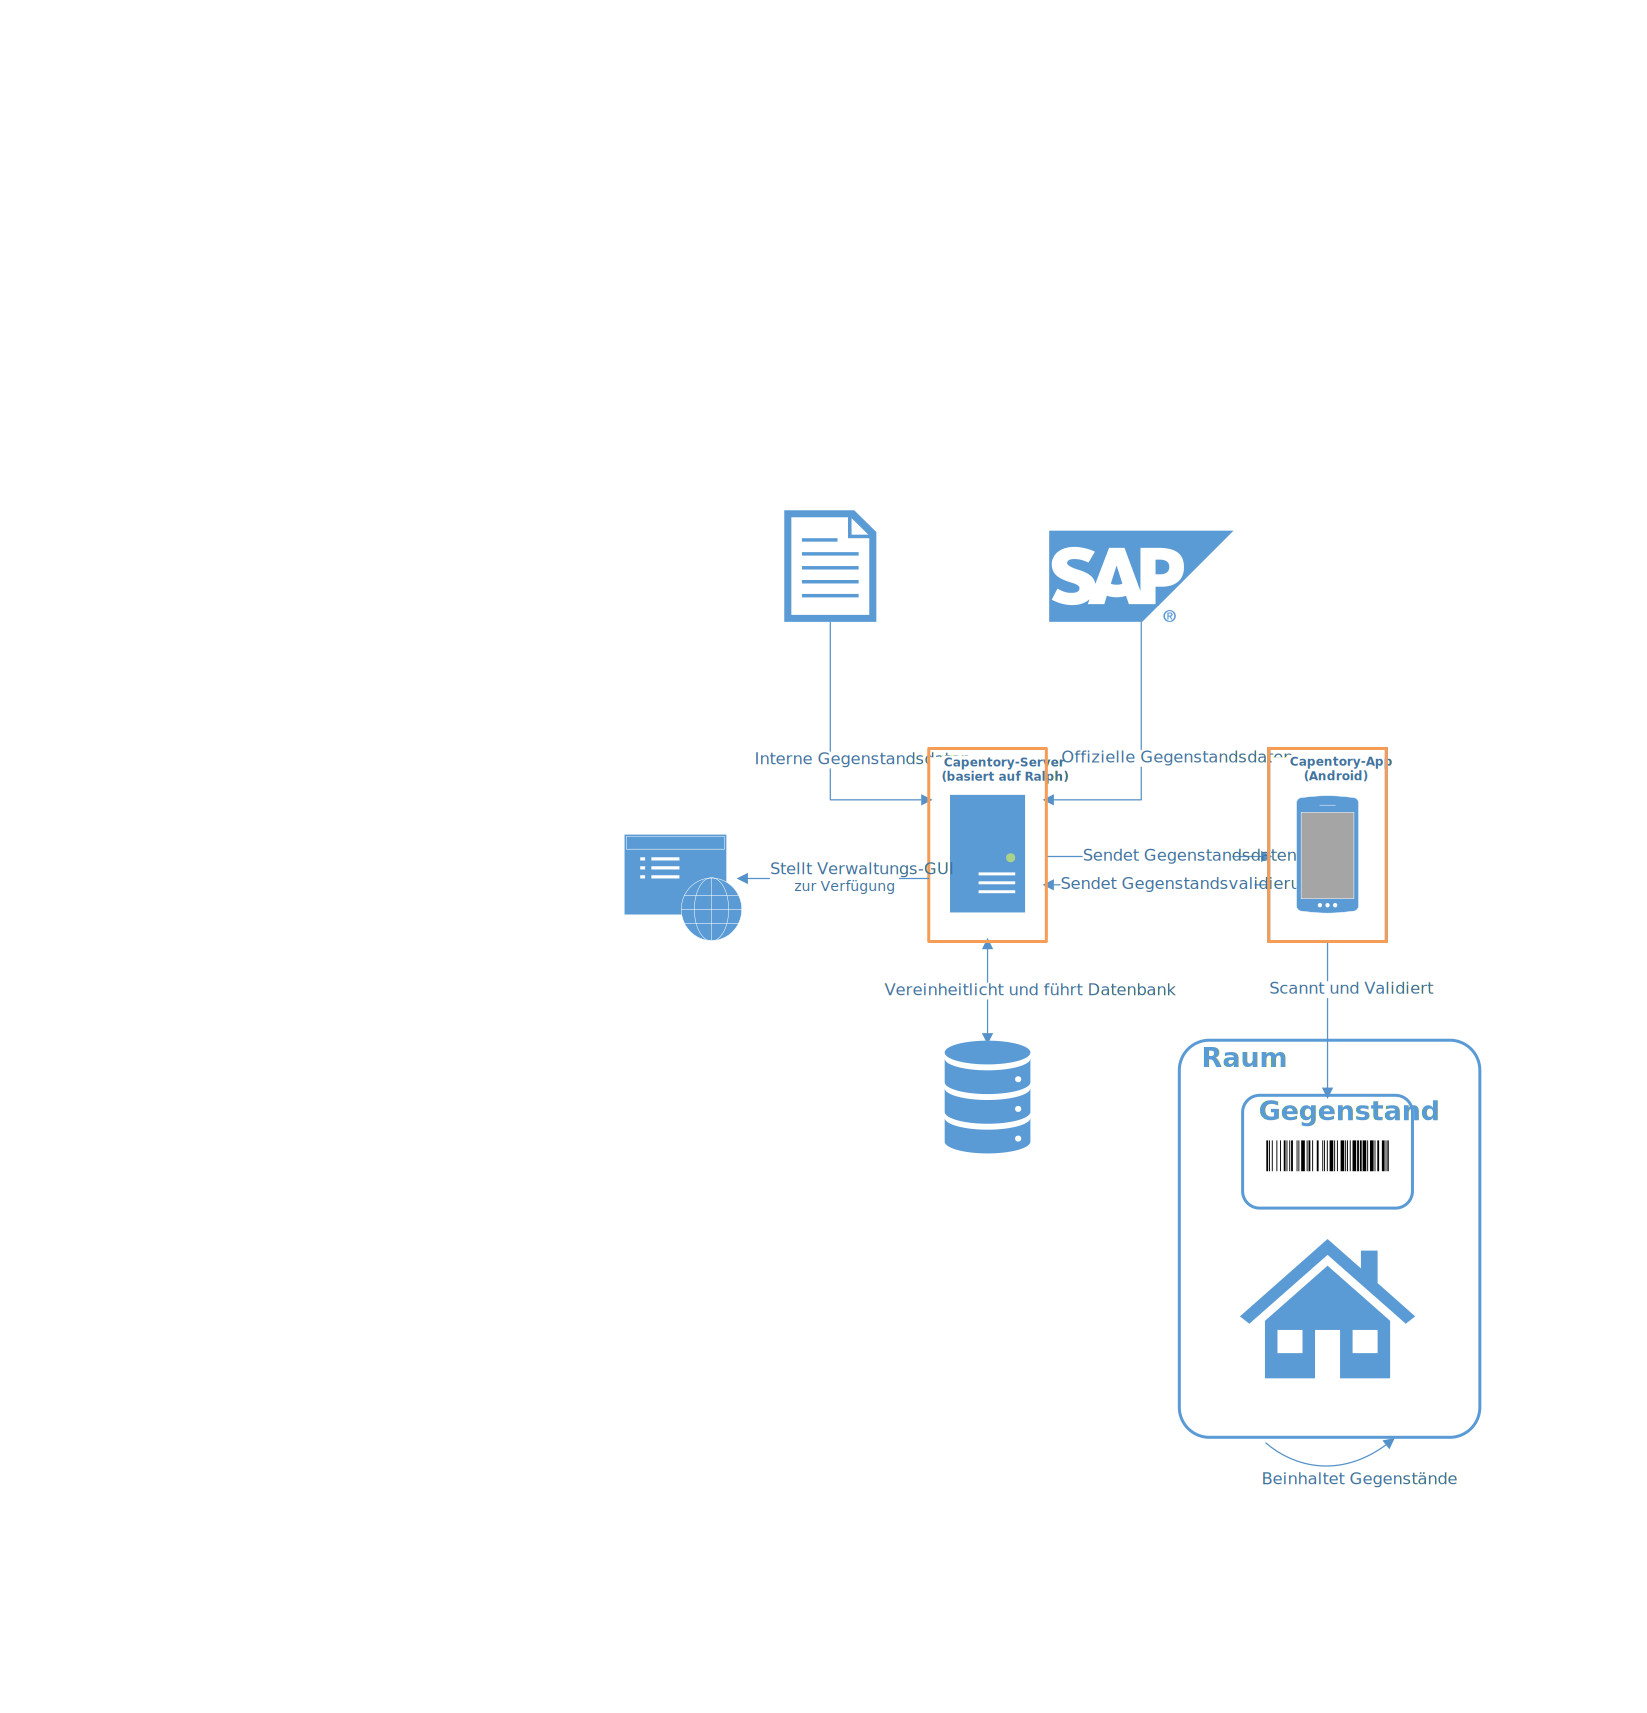
\includegraphics{bigpic.pdf}
  \caption{Übersicht und Funktionsgrafik zur Capentory-Infrastruktur
  \label{fig:gesamt}}
  \end{figure}

Das Ergebnis der vorliegenden Diplomarbeit kann vereinfacht durch die \abb{fig:gesamt} veranschaulicht werden. Die vorliegende Diplomarbeit kann dabei in drei Bereiche unterteilt werden. Die restlichen Kapitel erläutern die konkrete Implementierung und Funktionsweise dieser Bereiche: 


\begin{itemize}
  \tightlist
  \item
    Die Appsoftware (\kap{intro_app} bis \inkl \kap{das_scannen})
  \item
    Die Serversoftware (\kap{intro_server} bis \inkl \kap{die_zwei_module})
  \item
    Die Infrastruktur, auf der die Serversoftware ausgeführt wird (\kap{intro_infra})
\end{itemize}



%\chapter{Formatierung}

% wer hat diese Kapitel geschrieben oder leer
% \renewcommand{\kapitelautor}{Autor: Hans Huber}

%\input{text/demo_kap1.tex}

% wer hat diese Kapitel geschrieben oder leer
\chapter{Einführung in die App}
\label{intro_app}
\renewcommand{\kapitelautor}{Autor: Josip Domazet}

Das Ziel der Diplomarbeit ist es, eine App zu entwickeln, mit der man in
der Lage ist, eine Inventur durchzuführen. Um zu verstehen, wieso sich
das Projektteam für eine native App entschieden hat, muss man zwischen
zwei Begriffen unterscheiden \cite{native-vs-web}:

\begin{itemize}
\tightlist
\item
  Native App
\item
  Web-App
\end{itemize}

\hypertarget{nativ-versus-web}{%
\section{Nativ versus Web}\label{nativ-versus-web}}

Unter einer nativen App versteht man eine App, die für ein bestimmtes
Betriebssystem geschrieben wurde \cite{native-definition}. Eine Web-App
hingegen basiert auf HTML und wird per Browser aufgerufen. Sie stellt
nichts anderes als eine für mobile Geräte optimierte Website dar.

\hypertarget{begruxfcndung-fuxfcr-die-wahl-der-nativen-app}{%
\section{Begründung für die Wahl der nativen
App}\label{begruxfcndung-fuxfcr-die-wahl-der-nativen-app}}

Das Projektteam hat sich für eine native App entschieden. Um diese
Entscheidung nachvollziehen zu können, ist ein tieferer Einblick in den
gegebenen Use-Case erforderlich.

Das Ziel ist es nicht, möglichst viele Downloads im Play Store zu
erzielen oder etwaige Marketingmaßnahmen zu setzen. Es soll stattdessen
mit den gegebenen Ressourcen eine Inventurlösung entwickelt werden, die
die bestmögliche Lösung für die vorliegende Schule darstellt. Eine
native App wird eine Web-App hinsichtlich Qualität und User Experience
immer klar übertreffen.

Im vorliegenden Fall wäre es sicherlich möglich, eine Inventur mittels
Web-App durchzuführen, allerdings würde diese vor allem in den Bereichen
Performanz und Verlässlichkeit Mängel aufweisen. Diese zwei Bereiche
stellen genau die zwei Problembereiche dar, die es mit der vorliegenden
Gesamtlösung bestmöglich zu optimieren gilt. Des Weiteren bieten sich
native Apps ebenfalls für komplexe Projekte an, da Web-Apps aktuell noch
nicht in der Lage sind, komplexe Aufgabenstellungen mit vergleichbar
geringem Aufwand zu inkorporieren \cite{complex-article}. Die
vorliegende Arbeit ist dabei bereits allein aufgrund der in Betracht zu
ziehenden Sonderfälle als komplexe Aufgabenstellung einzustufen.

Unter Berücksichtigung dieser Gesichtspunkte wurde also der Entschluss
gefasst, eine native Applikation zu entwickeln, da diese ein insgesamt
besseres Produkt darstellen wird. Es sei gesagt, dass es auch hybride
Apps gibt. Diese sind jedoch einer nativen App in denselben Aspekten wie
eine Web-App klar unterlegen.

\hypertarget{auswahl-der-nativen-technologie}{%
\subsection{Auswahl der nativen
Technologie}\label{auswahl-der-nativen-technologie}}

Folgende native Alternativen waren zu vergleichen:

\begin{itemize}
\tightlist
\item
  Flutter \cite{flutter}
\item
  Xamarin \cite{xamarin}
\item
  Native IOS
\item
  Native Android (Java/Kotlin)
\end{itemize}

Flutter ist ein von Google entwickeltes Framework, dass eine gemeinsame
Codebasis für Android und IOS anbietet. Eine gemeinsame Codebasis wird
oftmals unter dem Begriff \texttt{cross-platform} zusammengefasst und
bedeutet, dass man eine mit Flutter entwickelte native App sowohl mit
Android-Geräten als auch mit IOS-Geräten verwenden kann. Flutter ist
eine relativ neue Plattform -- die erste stabile Version wurde erst im
Dezember 2018 veröffentlicht \cite{flutter-stable}. Außerdem verwendet
Flutter die Programmiersprache \texttt{Dart}, die Java ähnelt. Diese
Umstände sind ein Segen und Fluch zugleich. Flutter wird in Zukunft
sicherlich weiterhin an Popularität zulegen, allerdings ist die Anzahl
an verfügbarer Dokumentation für das junge Flutter im Vergleich zu den
anderen Optionen immer noch weitaus geringer.

Xamarin ist ebenfalls ein cross-platform Framework, das jedoch in C\#
geschrieben wird und älter (und damit bewährter) als Flutter ist.
Weiters macht Xamarin von der proprietären .NET-Platform Gebrauch.
Infolgedessen haben alle Xamarin-Apps Zugriff auf ein umfassendes
Repertoire von .NET-Libraries \cite{xamarin-details}. Da Xamarin und
.NET Microsoft angehören, ist eine leichtere Azure-Integration oftmals
ein Argument, das von offzielen Quellen verwendet wird. Xamarin wird --
anders als die restlichen Optionen -- bevorzugterweise in Visual Studio
entwickelt \cite{xamarin-vs}.

Native IOS wird nur der Vollständigkeit halber aufgelistet, stellte
allerdings zu keinem Zeitpunkt eine wirkliche Alternative dar, weil
IOS-Geräte einige Eigenschaften besitzen, die für eine Inventur nicht
optimal sind (\zB die Akkukapazität). Außerdem haben in etwa nur 20\%
aller Geräte \cite{ios-market-share} IOS als Betriebssystem und die
Entwicklung einer IOS-App wird durch strenge Voraussetzungen äußerst
unattraktiv gemacht. So kann man beispielsweise nur auf einem
Apple-Gerät IOS-Apps entwickeln.

\hypertarget{begruxfcndung-natives-android-java}{%
\subsubsection{Begründung: Natives Android
(Java)}\label{begruxfcndung-natives-android-java}}

Die Entscheidung ist schlussendlich auf natives Android (Java) gefallen.
Es mag zwar vielleicht nicht die innovativste Entscheidung sein, stellt
aber aus folgenden Gründen die bewährteste und risikoloseste Option dar:

\begin{itemize}
\tightlist
\item
  Natives Android ist eine allbekannte und weit etablierte Lösung. Die
  Wahrscheinlichkeit, dass die Unterstützung durch Google eingestellt
  wird, ist also äußerst gering.
\item
  Die App wird in den nächsten Jahren immer noch am Stand der Technik
  sein.
\item
  Natives Android hat mit großem Abstand die umfassendste Dokumentation.
\item
  An der Schule wird Java unterrichtet. Das macht somit eventuelle
  Modifikationen nach Projektabschluss durch andere Schüler viel
  einfacher möglich.
\item
  Dadurch, dass Kotlin erst seit 2019 \cite{kotlin-preference} offiziell
  die von Google bevorzugte Sprache ist, sind die meisten Tutorials
  immer noch in Java.
\item
  Sehr viele Unternehmen haben viele aktive Java-Entwickler. Dadurch
  wird die App attraktiver, da die Unternehmensmitarbeiter (von
  \zB allegro) keine neue Sprache lernen müssen, um Anpassungen
  durchzuführen.
\item
  Das Projektteam hat im Rahmen eines Praktikums bereits Erfahrungen mit
  nativem Java gesammelt.
\end{itemize}

Aus den Projektzielen hat sich in Absprache mit den Betreuern ergeben,
dass die App nicht auf jedem ``Steinzeitgerät'' zu funktionieren hat.
Das minimale API-Level der App ist daher 21 -- auch bekannt als Android
5.0 ``Lollipop''.

\hypertarget{einfuxfchrung-in-natives-java}{%
\section{Einführung in natives
Java}\label{einfuxfchrung-in-natives-java}}

Um eine Basis für die folgenden Kapitel zu schaffen, werden hier die
Basics der Android-Entwicklung mit nativem Java näher beschrieben.

\hypertarget{grundsuxe4tzliches}{%
\subsection{Grundsätzliches}\label{grundsuxe4tzliches}}

Das Layout einer App wird in XML Dateien gespeichert, während der
Programmcode in der Programmiersprache Java erstellt wird. Damit ist die
Entwicklung einer Android-App objektorientiert.

\hypertarget{single-activity-app}{%
\subsection{Single-Activity-App}\label{single-activity-app}}

Als Einstiegspunkt in eine App dient eine sogenannte \texttt{Activity}.
Eine Activity ist eine normale Java-Klasse, der durch Vererbung
UI-Funktionen verliehen werden.

Bis vor kurzem war es üblich, dass eine App mehrere Activities hat. Das
wird bei den Benutzern dadurch bemerkbar, dass die App \zB bei einem
Tastendruck ein weiteres Fenster öffnet, das das bisherige überdeckt.
Das neue Fenster ist eine eigene Activity. Google hat sich nun offiziell
für sogenannte Single-Activities ausgesprochen \cite{single-activity}.
Das heißt, dass es nur eine Activity und mehrere \texttt{Fragments}
gibt. Ein Fragment ist eine Teilmenge des UIs \bzw einer Activity.
Anstatt jetzt beim Tastendruck eine neue Activity zu starten, wird
einfach das aktuelle Fragment ausgetauscht. Dadurch, dass keine neuen
Fenster geöffnet werden, ist die User Experience (UX) um ein Vielfaches
besser -- die Performanz leidet nur minimal darunter. Die vorliegende
App ist aus diesen Gründen ebenfalls eine Single-Activity-App.

\chapter{Die Inventurlogik auf der App}
\label{inventurlogik_auf_der_app}

Die genaue Bedienung der App ist dem App-Handbuch zu entnehmen. Dieses
Kapitel befasst sich mit der Logik hinter einer Inventur.

\hypertarget{allgemeiner-ablauf-einer-inventur}{%
\section{Allgemeiner Ablauf einer
Inventur}\label{allgemeiner-ablauf-einer-inventur}}

Eine Inventur läuft immer wie folgt ab:

\begin{enumerate}
\def\labelenumi{\arabic{enumi}.}
\tightlist
\item
  Der Benutzer wählt die Inventur aus, an der er arbeiten will.
\item
  Der Benutzer wählt die Datenbanksicht aus. Dieser Schritt ist
  erforderlich, da die App auch mit der Ralph-Datenbanksicht kompatibel
  ist. An der Schule ist die HTL-Datenbanksicht auszuwählen.
\item
  Der Benutzer begibt sich zu einem Raum und wählt ihn auf der App aus.
\item
  Der Benutzer erhält die Gegenstandsliste für diesen Raum. Diese
  Gegenstandsliste gilt es abzuarbeiten.
\item
  Der Benutzer scannt die Barcodes der Gegenstände und arbeitet sie
  dadurch ab. Nicht aufgelistete Gegenstände werden automatisch ergänzt.
\item
  Der Benutzer kann auf Gegenstandsbasis Änderungen an den Feldern eines
  Gegenstandes vornehmen.
\item
  Wenn der Benutzer der Meinung ist, alle Gegenstände in diesem Raum
  erfasst zu haben, sendet er seine Validierungen an den Server.
\item
  Damit ist der ausgewählte Raum abgeschlossen und der Benutzer kann
  sich dem nächsten Raum annehmen.
\end{enumerate}

Alle Informationen, die die App bezieht, stammen vom Server.

\hypertarget{die-modelle}{%
\section{Die Modelle}\label{die-modelle}}

Um die Antworten des Servers abzubilden, wurden mehrere Modell-Klassen
erstellt. Folgende Modell-Klassen wurden angelegt:

\begin{itemize}
\tightlist
\item
  \texttt{Stocktaking}: Stellt eine Inventur dar.
\item
  \texttt{SerializerEntry}: Stellt eine Datenbanksicht dar.
\item
  \texttt{Room}: Stellt einen Raum dar.
\item
  \texttt{MergedItem}: Stellt einen Gegenstand dar.
\item
  \texttt{MergedItemField}: Stellt ein dynamisches Feld dar.
\item
  \texttt{Attachment}: Stellt einen Anhang dar.
\end{itemize}

\hypertarget{designgrundsuxe4tze}{%
\subsection{Designgrundsätze}\label{designgrundsuxe4tze}}

Eine Modell-Klasse verwaltet etwaige Statusinformationen immer selbst.
So weiß beispielsweise nur ein Gegenstand selbst, dass er ursprünglich
aus einem anderen Raum stammt. Dies verbessert die Lesbarkeit und
Wartbarkeit des Codes massiv, da diese Informationen abstrahiert sind
und nicht mehrmals an verschiendenen Stellen im Quellcode schlummern.

\hypertarget{die-fragments}{%
\section{Die Fragments}\label{die-fragments}}

Eine Inventur wird auf der App durch folgendene Fragments abgewickelt,
die gleichzeitig als Phasen verstanden werden können:

\begin{itemize}
\tightlist
\item
  \texttt{StocktakingFragment}
\item
  \texttt{RoomsFragment}
\item
  \texttt{ViewPagerFragment}

  \begin{itemize}
  \tightlist
  \item
    \texttt{MergedItemsFragment}
  \item
    \texttt{ValidatedMergedItemsFragment}
  \end{itemize}
\item
  \texttt{DetailedItemFragment}
\item
  \texttt{AttachmentsFragment}
\end{itemize}

\hypertarget{stocktakingfragment}{%
\paragraph{StocktakingFragment}\label{stocktakingfragment}}

ist das Fragment, in dem der Benutzer die aktuelle Inventur auswählt.
Die Inventur kann nur vom Administrator am Server angelegt werden.

Außerdem wählt der Benutzer hier die Datenbanksicht (``den Serializer'')
aus. Die App kommuniziert ausschließlich mittels REST API mit dem
Server. Diese Schnittstelle kann verschiedene Quellen haben. Die Quellen
sind abhängig von der ausgewählten Datenbanksicht.

Durch das Bestätigen eines langegezogenen blauen Buttons gelangt man
immer zur nächsten Inventurphase. In diesem Fall gelangt man zum
\texttt{RoomsFragment}.

\hypertarget{roomsfragment}{%
\paragraph{RoomsFragment}\label{roomsfragment}}

ist das Fragment, in dem der Benutzer den aktuellen Raum über eine
DropDown auswählt. Anstatt die DropDown zu verwenden, kann er alternativ
auch die Suchleiste verwenden. Als zusätzliche Alternative hat der
Benutzer die Möglichkeit den Barcode eines Raumes zu scannen. Nach der
Auswahl eines Raumes gelangt man zum \texttt{ViewPagerFragment}.

\hypertarget{viewpagerfragment}{%
\paragraph{ViewPagerFragment}\label{viewpagerfragment}}

ist das Fragment, das als Wrapper für das \texttt{MergedItemsFragment}
und das \texttt{ValidatedMergedItemsFragment} dient. Die einzige Aufgabe
dieses Fragments ist es, die zwei vorher genannten Fragments als Tabs
anzuzeigen. Dies wurde mit der neuen \texttt{ViewPager2}-Library
realisiert \cite{viewpager2}.

\hypertarget{mergeditemsfragment-validatedmergeditemsfragment}{%
\paragraph{MergedItemsFragment \&
ValidatedMergedItemsFragment}\label{mergeditemsfragment-validatedmergeditemsfragment}}

sind die Fragments, die die Gegenstandsliste eines Raumes verwalten und
sie dem Benutzer anzeigen. Das \texttt{MergedItemsFragment} zeigt dem
Benutzer die noch zu validierenden Gegenstände an. Das
\texttt{ValidatedMergedItemsFragment} erfüllt nur den Zweck, dem
Benutzer bereits validierte Gegenstände anzuzeigen und ihm die
Möglichkeit zu geben, validierte Gegenstände zurück zu den
nicht-validierten Gegenständen in \texttt{MergedItemsFragment} zu
verschieben. Daher trägt der Tab für das \texttt{MergedItemsFragment}
die Beschriftung ``TODO'', währenddessen der Tab für das
\texttt{ValidatedMergedItemsFragment} die Beschriftung ``DONE'' trägt.

Beide Fragments verwenden eine \texttt{RecyclerView}, um dem Benutzer
die Gegenstände anzuzeigen \cite{recyclerview}. Eine RecyclerView
generiert pro Eintrag ein Layout, hält aber nur die aktuell angezeigten
Einträge \inkl. Layout im RAM.

Die Gegenstände werden einzeln validiert. Durch das Scannen des Barcodes
eines Gegenstands (beziehungsweise durch das Klicken auf seine
GUI-Repräsentation) gelangt der Benutzer zum
\texttt{DetailedItemFragment}.

\hypertarget{detaileditemfragment}{%
\paragraph{DetailedItemFragment}\label{detaileditemfragment}}

ist das Fragment, das zur Validierung eines einzelnen Gegenstands dient.
Der Benutzer hat hier die Möglichkeit, etwaige Eigenschaften des
Gegenstandes (beispielsweise den Anzeigenamen) zu ändern. Ein Formular,
dass die Felder eines Gegenstandes beinhaltet, wird einmal angefordert
und anschließend für die gesamte Lebensdauer der App gespeichert. Anhand
dieses Formulars wird dann eine GUI-Repräsentation dynamisch erstellt.

Das Formular kann \texttt{ExtraFields} beinhalten. Das sind Felder, die
als nicht essentiel angesehen werden und infolgedessen standardmäßig
eingeklappt sind. Dazu gehören auch benutzerdefinierte Felder --
sognannte \texttt{CustomFields}. \texttt{ExtraFields} weisen ansonsten
dasselbe Verhalten wie herkömmliche Felder auf.

Folgende GUI-Komponenten wurden statisch implementiert, da sie Felder
repräsentieren, die unabhängig von der ausgewählten Datenbanksicht immer
vorhanden sind und daher nicht dynamisch sind:

\begin{itemize}
\tightlist
\item
  Ein read-only Textfeld für die Gegendstandsbeschreibung
\item
  Ein read-only Textfeld für den Barcode
\item
  Eine Checkbox ``Erst später entscheiden''
  (\siehe{das-stocktakingitem-modell})
\item
  Eine DropDown für Subrooms (\siehe{subrooms})
\end{itemize}

Man braucht für die gesamte Validierung eines Raumes -- insofern keine
Sonderfälle auftreten -- keine Verbindung zum Server. Der Benutzer kann
die Gegenstandsliste an einer Lokalität mit einer guten Verbindung
anfordern, den Raum mit schlechter Verbindung betreten und alle
Gegenstände validieren. Anschließend kann er den Raum verlassen und
seine Validierungen an den Server senden. Damit wird der Bedarf an
Netzwerkanfragen in Räumen mit schlechter Netzwerkverbindung minimiert.

Der Benutzer kann zusätzlich zur Validierung auch Anhänge für einen
Gegenstand definieren, dazu landet er beim \texttt{AttachmentsFragment}.

\hypertarget{attachmentsfragment}{%
\paragraph{AttachmentsFragment}\label{attachmentsfragment}}

ist das Fragment, das die Anhänge eines Gegenstandes verwaltet. Der
Benutzer sieht hier die bereits vorhandenen Anhänge mit Beschriftungen
und kann weitere Anhänge hinzufügen. Bilder werden direkt angezeigt.
Andere Dateien werden hingegen als Hyperlink dargestellt. Der Benutzer
kann diese per Browser runterladen. Zum Hochladen eigener Anhänge greift
die App auf den Standard-Dateibrowser des Systems zurück.

Das Outsourcen auf Webbrowser und Dateibrowser bietet den massiven
Vorteil, dass man sich die Entwicklung eigener Download-Manager
\bzw File-Manager erspart und auf Apps setzen kann, die von namenhaften
Herstellern entwickelt werden. Fast jedes System hat bereits beide
Komponenten vorinstalliert, daher treten bezüglich der Verfügbarkeit
keine Probleme auf.

Beim dem Hochladen von Bildern komprimiert die App jene zuvor. Zur
Kompression wird das \texttt{WEBP}-Format verwendet, das dem
mittlerweile veralteten \texttt{JPG}-Standard überlegen ist \cite{webp}.
Die Qualität des Bildes ist einstellbar:

\begin{itemize}
\tightlist
\item
  100 \% (keine Kompression)
\item
  95 \%
\item
  85 \%
\item
  75 \%
\end{itemize}

Der Server speichert den gesendeten Anhang nur einmal (Dateien werden
anhand von Hashes unterschieden). Wenn ein Benutzer allen PCs in einem
EDV-Saal dasselbe Bild zuweist, wird es nur einmal am Server hinterlegt.
Die Anzahl der Anhänge ist nicht limitiert.

\hypertarget{validierungslogik}{%
\section{Validierungslogik}\label{validierungslogik}}

\texttt{MergedItemsFragment} \& \texttt{DetailedItemFragment} sind die
Fragments, die den Großteil einer Inventur ausmachen. Der Benutzer
scannt alle SAP-Barcodes, die sich in einem Raum befinden. Im Idealfall
entspricht diese Menge exakt der Menge der Gegenstände, die dem Benutzer
im \texttt{MergedItemsFragment} angezeigt wird. Im Normalfall wird dies
durch etwaige Sonderfälle jedoch nicht gegeben sein. Nach dem Scannen
eines Gegenstandes werden die Felder des Gegenstandes dem Benutzer im
\texttt{DetailedItemFragment} angezeigt. In diesem Fragment hat der
Benutzer zwei Buttons, mit denen er den Gegenstand validieren kann:

\begin{itemize}
\tightlist
\item
  \textbf{Grüner Button}: Mit diesem Button wird signalisiert, dass sich
  der Gegenstand im Raum befindet und der Gegenstand wird mitsamt
  etwaigen Änderungen an seinen Attributen/Feldern übernommen. Dazu wird
  ein \texttt{ValidationEntry} erstellt. Alternativ kann der Benutzer
  das Klicken dieses Buttons mit dem Schütteln des Gerätes ersetzen. Die
  Schüttel-Sensibilität ist über die Einstellungen konfigurierbar (und
  auch deaktivierbar).
\item
  \textbf{Roter Button}: Mit diesem Button wird signalisiert, dass sich
  der Gegenstand nicht im Raum befindet. Dieser Button wird im
  Normalfall nie betätigt werden, da ein Gegenstand, der sich nicht in
  diesem Raum befindet, nicht gescannt werden kann und daher dieses
  Fenster nie geöffnet werden wird. Der Button hat trotzdem einen Sinn,
  da der Benutzer damit die ``TODO''-Liste über das GUI verkleinern
  kann, um sich einen besseren Überblick zu verschaffen.
\end{itemize}

\hypertarget{der-validationentry}{%
\subsection{Der ValidationEntry}\label{der-validationentry}}

Ein \texttt{ValidationEntry} beinhaltet sämtliche Informationen, die der
Server benötigt, um die Datensätze eines Gengenstandes entsprechend
anzupassen, und stellt eine Gegenstandsvalidierung dar. Ein
\texttt{ValidationEntry} beinhaltet immer den Primary Key eines
Gegenstandes und die Felder, die sich geändert haben. Ein
\texttt{ValidationEntry} hat daher eine Liste an Feldern
\texttt{List\textless{}Field\textgreater{}}. Wenn sich der Wert eines
Feldes geändert hat, wird diese Liste um einen Eintrag erweitert.

Da die Felder wie erwähnt dynamisch (und dadurch generisch) sind, wurden
Java Generics eingesetzt \cite{java-generics}, um diese abbilden zu
können. \texttt{Field} ist eine innere Klasse in
\texttt{ValidationEntry}:

\begin{Shaded}
\begin{Highlighting}[]
\KeywordTok{public} \DataTypeTok{static} \KeywordTok{class} \BuiltInTok{Field}\NormalTok{<T> \{}
    \KeywordTok{private} \BuiltInTok{String}\NormalTok{ fieldName;}
    \KeywordTok{private}\NormalTok{ T fieldValue;}
\NormalTok{    ...}
\end{Highlighting}
\end{Shaded}

Ein Feld besteht also immer aus einem Feldnamen und einem generischen
Feldwert.

\hypertarget{sendeformat}{%
\subsubsection{Sendeformat}\label{sendeformat}}

Das \texttt{MergedItemsFragment} (\bzw das \texttt{MergedItemsViewModel}
\siehe{die_app_architektur}) verfügt über eine \texttt{HashMap}
(\texttt{Map\textless{}MergedItem,\ List\textless{}ValidationEntry\textgreater{}\textgreater{}}),
die alle \texttt{ValidationEntries} beinhaltet. Einem Gegenstand ist
eine Liste an \texttt{ValidationEntries} zugeordnet, da Subitems eigene
\texttt{ValiditionEntries} bekommen können
(\siehe{sonderfuxe4lle-auf-der-app}).

Wenn ein Raum abgeschlossen ist, werden alle \texttt{ValidationEntries}
in einer Liste vereint und anschließend in eine JSON-Darstellung
transformiert. Dieses JSON wird dem Server gesandt und damit ist der
aktuelle Raum abgeschlossen. Der Benutzer kann sich nun den restlichen
Räumen annehmen. Die genaue Kommunikationsarchitektur wird im Kapitel
\protect\hyperlink{das-repository-im-detaila}{``Das Repository im
Detail''} beschrieben (\siehe{das-repository-im-detail}).

Der Server erstellt auf Basis der gesendeten \texttt{ValidationEntries}
Änderungsvorschläge -- sogenannte \texttt{Change\ Proposals}
(\siehe{uxe4nderungsvorschluxe4ge}). Das \texttt{POST}-Format wird im
Kapitel \protect\hyperlink{json-schema}{``JSON-Schema''} beschrieben
(\siehe{json-schema}).

\hypertarget{quickscan}{%
\subsection{QuickScan}\label{quickscan}}

Der häufigste Fall einer Inventur wird jener sein, dass ein Gegenstand
im richtigen Raum ist und der Benutzer ohne weiteren Input auf den
grünen Button drückt. Da dies einen unnötigen Overhead darstellt, wurde
die App um den \texttt{QuickScan}-Modus erweitert. Hierbei wird sofort
nach dem Scannen ein \texttt{ValidationEntry} erstellt, ohne dass zuvor
das \texttt{DetailedItemFragment} geöffnet wird. Dieser Modus ist durch
einen Button im \texttt{MergedItemsFragment} aktivierbar/deaktivierbar.

Falls ein Sonderfall auftreten sollte, vibriert das Gerät zweimal und
öffnet doch das \texttt{DetailedItemFragment}. Damit wird gewährleistet,
dass der Benutzer nicht irrtümlich mit dem Scannen weitermacht. Er muss
diesen Sonderfall händisch validieren. Haptisches Feedback ist für
Sonderfälle reserviert.

\hypertarget{sonderfuxe4lle-auf-der-app}{%
\subsection{Sonderfälle auf der App}\label{sonderfuxe4lle-auf-der-app}}

Ein zentrales Thema der vorliegenden Diplomarbeit ist die Behandlung der
Sonderfälle.

\hypertarget{subitems}{%
\subsubsection{Subitems}\label{subitems}}

Wenn sich mehrere physische Gegenstände einen Barcode teilen, werden sie
in der primären Liste lediglich durch einen einzelnen Eintrag
abgebildet. Ein Eintrag des Serversystems kann also mehrere Subitems
zusammenfassen.

Der Server inkludiert in seiner Antwort für jeden Gegenstand einen
Zähler, der die nötigen Informationen zur Behandlung dieses Sonderfalles
beinhaltet. Der Zähler wird in weiterer Folge
\texttt{times\_found\_last}-Zähler genannt. Falls ein Gegenstand aus
mehreren Subitems bestehen sollte, ist der
\texttt{times\_found\_last}-Zähler in der Antwort des Servers größer als
1. Dieser Counter wird dem Benutzer in folgender Form angezeigt:
\texttt{{[}Anzahl\ aktuell\ gefunden{]}\ /\ {[}Anzahl\ zuletzt\ gefunden{]}}.

Bei der Validierung eines Subitems wird ein eigener
\texttt{ValidationEntry} erstellt und die Anzahl der aktuellen Funde
erhöht. \texttt{Change\ Proposals} (\siehe{uxe4nderungsvorschluxe4ge}),
die auf Basis dieser \texttt{ValidationEntries} erstellt werden, werden
dem echten ``Parent''-Gegenstand zugeordnet und können wahlweise
angewandt werden.

Falls ein Gegenstand mehrmals gescannt wird, wird -- nach Bestätigung
durch den Benutzer -- die Anzahl der aktuellen Funde erhöht und wiederum
einen \texttt{ValidationEntry} erstellt, selbst wenn es sich bei dem
Gegenstand aktuell nicht um ein Subitem handelt.

\hypertarget{subrooms}{%
\subsubsection{Subrooms}\label{subrooms}}

Subrooms sind logische Räume in einem Raum (\zB steht ein PC in einem
Kasten, der wiederum in einem Raum steht). Subrooms werden dem Benutzer
im \texttt{MergedItemsFragment} als einklappbare Zwischenebenen, denen
Gegenstände zugeordnet sind, angezeigt. Die Subroom-Zugehörigkeit kann
auf Gegenstandsbasis über eine DropDown geändert werden. Die
Subroom-Zugehörigkeit wird in einem \texttt{ValidationEntry} immer
gesetzt, auch wenn sie sich nicht geändert hat.

Die Gegenstandsliste des \texttt{MergedItemsFragment} beinhaltet in
Wahrheit auch die Subrooms. Dies ist notwendig, da die
\texttt{RecyclerView}, die dazu genutzt wird dem Benutzer die
Gegenstände anzuzeigen, keine Möglichkeit bietet, eine Hierarchie
\bzw Zwischenebenen darzustellen. Daher implementieren das
\texttt{Room}-Modell und das \texttt{MergedItem}-Modell das Interface
\texttt{RecyclerViewItem} und die RecyclerView erhält eine Liste an
\texttt{RecyclerViewItems} - dies ist ein typisch polymorpher Ansatz.
Abhängig vom Typen des aktuellen Listenelements baut die RecyclerView
entweder ein Gegenstandslayout oder ein Raumlayout auf. Die Anzahl der
Subrooms ist weder in der Tiefe noch in der Breite limitiert.

\hypertarget{unbekannte-gegenstuxe4nde}{%
\subsubsection{Unbekannte Gegenstände}\label{unbekannte-gegenstuxe4nde}}

Falls ein Gegenstand, der sich nicht in der aktuellen Gegenstandsliste
befindet, gescannt wird, muss der Server dazu befragt werden. Es gibt
zwei mögliche Antwortszenarien. Die \texttt{ValidationEntries} für diese
Sonderfälle unterscheiden sich nicht von den bisherigen.

\hypertarget{neuer-gegenstand}{%
\subparagraph{Neuer Gegenstand}\label{neuer-gegenstand}}

Der Gegenstand befindet sich überhaupt nicht in der Datenbank. Im
``DONE''-Tab haben solche Gegenstände eine blaue Hervorhebung.

\hypertarget{gegenstand-aus-anderem-raum}{%
\subparagraph{Gegenstand aus anderem
Raum}\label{gegenstand-aus-anderem-raum}}

Der Gegenstand befindet in der Datenbank und stammt ursprünglich aus
einem anderen Raum. Im ``DONE''-Tab haben solche Gegenstände eine orange
Hervorhebung.

\chapter{Die App-Architektur}
\label{die_app_architektur}

Die App muss ein verlässliches und vorhersehbares Verhalten aufweisen.
Die vom Benutzer erstellten Validierungen dürfen beispielsweise nicht
einfach verschwinden. Um das zu gewährleisten, ist eine durchdachte
App-Architektur vonnöten. Da die App-Architektur ein sehr zeitintensiver
und zentraler Aspekt der vorliegenden Diplomarbeit ist, der als
Fundament für die eigentlichen Ziele dient, folgt nun eine ausführliche
Erläuterung.

\hypertarget{separation-of-concerns}{%
\section{Separation of Concerns}\label{separation-of-concerns}}

In Android ist es eine äußerst schlechte Idee, sämtliche Logik in einer
Activity oder einem Fragment zu implementieren. Das softwaretechnische
Prinzip \texttt{Separation\ of\ Concerns\ (SoC)} hat unter Android einen
besonderen Stellenwert. Dieses Prinzip beschreibt im Wesentlichen, dass
eine Klasse nur einer Aufgabe dienen sollte. Falls eine Klasse mehrere
Aufgaben erfüllt, so muss diese auf mehrere logische Komponenten
aufgeteilt werden. Beispiel: Eine Activity \bzw ein Fragment hat immer
die Verantwortung, die Kommunikation zwischen UI und Benutzer
abzuwickeln. Bad Practice wäre es, wenn eine Activity ebenfalls dafür
verantwortlich ist, Daten von einem Server abzurufen.

Das Prinzip verfolgt das Ziel, die
\texttt{God\ Activity\ Architecture\ (GAA)} möglichst zu vermeiden
\cite{god-activities}. Eine God-Activity ist unter Android eine
Activity, die die komplette Business-Logic beinhaltet und \texttt{SoC}
in jeglicher Hinsicht widerspricht. God-Activities gilt es dringlichst
zu vermeiden, da sie folgende Nachteile mit sich bringen:

\begin{itemize}
\tightlist
\item
  Refactoring wird kompliziert
\item
  Wartung und Dokumentation werden äußerst schwierig
\item
  Automatisiertes Testing (\zB Unit-Testing) wird nahezu unmöglich
  gemacht
\item
  Größere Bug-Anfälligkeit
\item
  Im Bezug auf Android gibt es oftmals massive Probleme mit der
  Konsistenz einer Activity -- da eine Activity und ihre Daten schnell
  vernichtet werden können (\zB wenn der Benutzer sein Gerät rotiert und
  das Gerät den Bildschirmmodus wechselt,
  \siehe{das-fragment-und-das-viewmodel-im-detail})
\end{itemize}

God-Activities sind ein typisches Beispiel für Spaghetticode.

Als Reaktion auf eine Vielzahl von Apps, die Probleme mit God-Activites
aufwiesen, hat Google Libraries veröffentlicht, die klar auf eine
MVVM-Architektur abzielen \cite{mvvm}. Daher fiel die Wahl der
App-Architektur auf MVVM.

\hypertarget{designgrundlagen-von-mvvm}{%
\section{Designgrundlagen von MVVM}\label{designgrundlagen-von-mvvm}}

MVVM steht für Model-View-Viewmodel \cite{mvvm-wiki}. Wie man am Namen
bereits erkennt, gilt es zwischen drei Komponenten/Ebenen zu
unterscheiden \cite{mvvm-article}.

\hypertarget{model}{%
\paragraph{Model}\label{model}}

Model beschreibt die Ebene der Daten und wird daher oftmals auch als
Datenzugriffsschicht bezeichnet. Diese Ebene beinhaltet so viel
Anwendungslogik wie möglich.

\hypertarget{view}{%
\paragraph{View}\label{view}}

View beschreibt die graphische Ebene und umfasst daher das GUI. Diese
Ebene soll so wenig Logik wie möglich beinhalten.

\hypertarget{viewmodel}{%
\paragraph{ViewModel}\label{viewmodel}}

Das ViewModel dient als Bindeglied zwischen dem Model und der View. Die
Logik der View wird in diese Ebene hinaufverschoben.

\hypertarget{mvvm-in-android}{%
\section{MVVM in Android}\label{mvvm-in-android}}

Mit der Einführung der \texttt{Architecture\ Components} hat Google
Android-Entwicklern eine Vielzahl an Libraries zur Verfügung gestellt,
um MVVM leichter in Android implementieren zu können
\cite{mvvm-architecture-components}. Die konkrete Implementierung in
Android ist in Abbildung \abb{fig:mvvm} ersichtlich.

\begin{figure}
\centering
\includegraphics[width=2.60417in,height=\textheight]{mvvm.png}
\caption{MVVM in Android nach Google \cite{mvvm} \cite{mvvm-bild}
\label{fig:mvvm}}
\end{figure}

In dem vorliegenden Fall ist unser \texttt{Fragment} die \texttt{View},
das \texttt{Repository} das \texttt{Model} und das \texttt{ViewModel}
ist in Android namensgleich. MVVM ist streng hierarchisch. Wie in der
Abbildung zu erkennen ist, kommuniziert jede Ebene nur mit der
hierarchisch nächsten Ebene.

\hypertarget{das-repository-im-detail}{%
\subsection{Das Repository im Detail}\label{das-repository-im-detail}}

Wie in der \abb{fig:mvvm} veranschaulicht, ist das Repository alleinig
dafür zuständig, Daten vom Server anzufordern. Beispielsweise wird die
Gegenstandsliste für einen Raum vom Repository angefordert -- und von
keiner anderen Ebene. Die Kommunikation zwischen der App und dem Server
findet ausschließlich im \texttt{JSON}-Format statt. JSON ist ein
text-basiertes und kompaktes Datenaustauschformat
\cite{json-format-doku}.

Das Repository fordert JSON an und instanziiert anschließend anhand der
Serverantwort Objekte der Modell-Klassen (\siehe{die-modelle}). Das
Repository ist die einzige Ebene, die mit den rohen JSON-Antworten des
Servers arbeitet. Die restlichen Ebenen arbeiten mit den abstrahierten
Objekten, also \zB mit \texttt{MergedItems} oder \texttt{Rooms}.

Die Kommunikation zwischen dem Server und der App wird mit zwei
Libraries abgewickelt:

\begin{itemize}
\tightlist
\item
  Volley
\item
  Retrofit
\end{itemize}

\hypertarget{jsonrequest-volley}{%
\subsubsection{JsonRequest (Volley)}\label{jsonrequest-volley}}

Android bietet Entwicklern eine Out-of-the-box Netzwerklibrary namens
\texttt{Volley} an, mithilfe derer man unter anderem JSON-Anfragen
verarbeiten kann \cite{volley}. Da diese für die vorliegenden Zwecke
nicht komplett geeignet war, hat das Diplomarbeitsteam die gegebene
Library durch den Einsatz von Vererbung und einer Wrapper-Klasse
modifiziert. Die Library wurde in folgenden Punkten angepasst:

\begin{itemize}
\tightlist
\item
  Im Falle eines Fehlers wird die Anfrage wiederholt (Ausnahme:
  Zeitüberschreitungsfehler). Die maximale Anzahl an Wiederholungen ist
  limitiert.
\item
  Die maximale Timeout-Dauer wurde erhöht.
\item
  Leere Antworten werden von der App als valide Antwort behandelt und
  können ohne Fehler verarbeitet werden.
\item
  Im Header der Anfrage wird der Content-Type der Anfrage auf JSON
  festgelegt.
\item
  Im Header wird das zur Authentifikation notwendige API-Token
  mitgeschickt. Die Authentifizierung ist über einen Parameter
  deaktivierbar.
\item
  Im Header wird die Systemsprache des Clients als standardisierter
  ISO-639-Code mitgesendet. Der Server passt seine Antwort auf die
  verwendete Sprache an \cite{ISO-639}. Die Bezeichnung der Felder, die
  dem Benutzer auf Gegenstandsbasis angezeigt werden, ist beispielsweise
  abhängig von der Systemsprache.
\item
  Zum Zeitpunkt der Anfrage ist nicht bekannt, ob die Antwort als
  \texttt{JSONArray} (\zB für eine Gegenstandsliste) oder als
  \texttt{JSONObject} (\zB für einen explizit angefragten Gegenstand)
  erfolgen wird. Da das Backend abhängig von der Anfrage sowohl mit
  einem \texttt{JSONArray} als auch einem \texttt{JSONObject} antworten
  kann, ist der Rückgabewert der Netzwerkanfrage immer ein String. Die
  Umwandlung erfolgt erst im Repository. Dies führt zu keinen
  Perfomance-Problemen, da die vorgefertigte Android Library den String
  zwar zu einem früheren Zeitpunkt aber auf dieselbe Weise umwandeln
  würde.
\end{itemize}

Diese Anpassungen wurden aus zwei Gründen vorgenommen:

\begin{itemize}
\tightlist
\item
  Um eine robustere Netzwerklibrary zu erhalten, die es ermöglicht in
  Räumen mit Netzwerkproblemen dennoch eine Inventur durchzuführen.
\item
  Um eine spätere Abstraktion der Netzwerkanfragen durchführen zu können
  (\siehe{konkrete-mvvm-implementierung}).
\end{itemize}

Sämtliche Netzwerkanfragen (die Raumliste, die Gegenstandsliste etc.)
werden mit der modifizierten \texttt{Volley}-Library durchgeführt. Die
einzige Ausnahme sind hierbei die Anhänge (\siehe{retrofit}).

\hypertarget{jsonrequest-beispiel}{%
\subsubsection{JsonRequest -- Beispiel}\label{jsonrequest-beispiel}}

Eine Anfrage wird nie direkt, sondern immer über einen Wrapper
ausgeführt. Der Konstruktor ist wie folgt aufgebaut:

\begin{itemize}
\tightlist
\item
  \texttt{Context\ context}: Ist eine Schnittstelle, die globale
  Information über die App-Umgebung zur Verfügung stellt \cite{context}
  und von Android zur Verfügung gestellt wird. Jede UI-Komponente
  (\zB Textfelder, Buttons, Fragments, etc.) verfügt über einen Context.
  Ein besonderer Context ist der globale Application-Context. Dieser ist
  einzigartig und ist ein \texttt{Singleton}. Ein Singleton bedeutet,
  dass von einer Klasse nur ein (globales) Objekt besteht
  \cite{singleton}.
\item
  \texttt{int\ method}: Ist die HTTP-Methode. Die App verwendet
  \texttt{GET}, \texttt{OPTIONS} und \texttt{POST}.
\item
  \texttt{String\ url}: Ist die URL, die eine JSON-Antwort liefern soll.
\item
  \texttt{@Nullable\ String\ requestBody}: Eventuelle Parameter, die an
  den Server gesendet werden sollen. Dieser Paramter ist für einen
  \texttt{POST}-Request wichtig.
\item
  \texttt{NetworkSuccessHandler\ successHandler}: Funktionales Interface
\item
  \texttt{NetworkErrorHandler\ errorHandler}: Funktionales Interface
\end{itemize}

Ein Request kann wie folgt ausschauen:

\begin{Shaded}
\begin{Highlighting}[]
\NormalTok{RobustJsonRequestExecutioner robustJsonRequestExecutioner =}
 \KeywordTok{new} \FunctionTok{RobustJsonRequestExecutioner}\NormalTok{(context, }\BuiltInTok{Request}\NormalTok{.}\FunctionTok{Method}\NormalTok{.}\FunctionTok{GET}\NormalTok{,}
  \StringTok{"https://www.beispiel.org/"}\NormalTok{, }\KeywordTok{null}\NormalTok{, }
\NormalTok{  payload -> \{}
         \CommentTok{// }\AlertTok{TODO}\CommentTok{: Antwort verarbeiten}
         \CommentTok{// -> Anhand der Antwort Modell-Objekte instanziieren}
\NormalTok{     \},}
\NormalTok{  error -> \{}
         \CommentTok{// }\AlertTok{TODO}\CommentTok{: Fehler verarbeiten}
\NormalTok{     \});}
     
\NormalTok{ robustJsonRequestExecutioner.}\FunctionTok{launchRequest}\NormalTok{();}
\end{Highlighting}
\end{Shaded}

Wie man sehen kann, sind die letzten beiden Parameter funktionale
Interfaces, die dazu dienen, Methoden als Parameter übergeben zu können.
Ein Interface mit einer einzigen abstrakten Methode ist als funktionales
Interface zu bezeichnen \cite{lambda}. Da Android Studio Java 8 Language
Features unterstützt, verwendet die App mehrheitlich Lambda-Ausdrücke
\cite{java8}. Lambda-Ausdrücke sind im Wesentlichen dazu da, funktionale
Interfaces in vereinfachter Schreibweise verwenden zu können. Da es nur
eine einzige abstrakte Methode gibt, kann die Schreibweise simplifiziert
werden, weil klar ist, von welcher Methode die Rede ist. Damit fallen --
wie im obigen Beispiel zu sehen -- redundante Informationen wie
Rückgabetyp und Methodenkörper vollständig weg. Das obige Beispiel würde
ohne Lambda-Ausdrücke wie folgt ausschauen:

\begin{Shaded}
\begin{Highlighting}[]
\NormalTok{RobustJsonRequestExecutioner robustJsonRequestExecutioner = }
 \KeywordTok{new} \FunctionTok{RobustJsonRequestExecutioner}\NormalTok{(context, }\BuiltInTok{Request}\NormalTok{.}\FunctionTok{Method}\NormalTok{.}\FunctionTok{GET}\NormalTok{, }
 \StringTok{"https://www.beispiel.org/"}\NormalTok{, }\KeywordTok{null}\NormalTok{,}
     \KeywordTok{new} \FunctionTok{NetworkSuccessHandler}\NormalTok{() \{}
         \AttributeTok{@Override}
         \KeywordTok{public} \DataTypeTok{void} \FunctionTok{handleSuccess}\NormalTok{(}\BuiltInTok{String}\NormalTok{ payload) \{}
             \CommentTok{// }\AlertTok{TODO}\CommentTok{: Antwort verarbeiten}
             \CommentTok{// -> Anhand der Antwort Modell-Objekte instanziieren}
\NormalTok{         \}}
\NormalTok{     \},}
     \KeywordTok{new} \FunctionTok{NetworkErrorHandler}\NormalTok{() \{}
         \AttributeTok{@Override}
         \KeywordTok{public} \DataTypeTok{void} \FunctionTok{handleError}\NormalTok{(}\BuiltInTok{Exception}\NormalTok{ error) \{}
             \CommentTok{// }\AlertTok{TODO}\CommentTok{: Fehler verarbeiten}
\NormalTok{         \}}
\NormalTok{     \});}

\NormalTok{robustJsonRequestExecutioner.}\FunctionTok{launchRequest}\NormalTok{();}
\end{Highlighting}
\end{Shaded}

Lambdas sind eine Option, um \texttt{Callbacks} in Java zu
implementieren. Ein Callback (``Rückruffunktion'') ist eine Methode, die
einer anderen Methode als Parameter übergeben werden kann. Die soeben
erwähnten funktionalen Interfaces sind typische Callbacks
\cite{Callbacks}. Es gibt zwei Arten von Callbacks:

\begin{itemize}
\tightlist
\item
  Synchrone Callbacks: Die Ausführung der übergebenen Methode erfolgt
  sofort.
\item
  Asynchrone Callbacks: Die Ausführung der übergebenen Methode erfolgt
  zu einem späteren Zeitpunkt.
\end{itemize}

In diesem Fall wird die Methode \texttt{handleSuccess} aufgerufen,
sobald der Client die Antwort erhalten hat. Damit handelt es sich um ein
asynchrones Callback. Callbacks werden in der App sehr häufig
eingesetzt.

\hypertarget{retrofit}{%
\subsubsection{Retrofit}\label{retrofit}}

\texttt{Retrofit} ist eine weitere Netzwerk-Library (\bzw Libraries),
die das Projektteam eingesetzt hat. Retrofit wurde nur zum Senden von
Dateien eingesetzt, weil dies mit Volley nur erschwert möglich ist. Mit
dieser Library wurde die Anhang-Funktion realisiert.

Das Projektteam hat bei dem einzigen die bereits bekannte Callback-Logik
verwendet:

\begin{Shaded}
\begin{Highlighting}[]
\NormalTok{Call<}\BuiltInTok{String}\NormalTok{> call = }\FunctionTok{prepareCall}\NormalTok{(args);}
\NormalTok{call.}\FunctionTok{enqueue}\NormalTok{(}\KeywordTok{new} \BuiltInTok{Callback}\NormalTok{<}\BuiltInTok{String}\NormalTok{>() \{}
    \AttributeTok{@Override}
    \KeywordTok{public} \DataTypeTok{void} \FunctionTok{onResponse}\NormalTok{(Call<}\BuiltInTok{String}\NormalTok{> call, }\BuiltInTok{Response}\NormalTok{<}\BuiltInTok{String}\NormalTok{> response) \{}
        \CommentTok{// }\AlertTok{TODO}\CommentTok{: Antwort verarbeiten}
        \CommentTok{// -> Anhand der Antwort Modell-Objekte instanziieren}
\NormalTok{    \}}
    \AttributeTok{@Override}
    \KeywordTok{public} \DataTypeTok{void} \FunctionTok{onFailure}\NormalTok{(Call<}\BuiltInTok{String}\NormalTok{> call, }\BuiltInTok{Throwable}\NormalTok{ t) \{}
        \CommentTok{// }\AlertTok{TODO}\CommentTok{: Fehler verarbeiten}
\NormalTok{    \}}
\NormalTok{\});}
\end{Highlighting}
\end{Shaded}

In Retrofit werden API-Endpunkte über Interfaces definiert:

\begin{Shaded}
\begin{Highlighting}[]
\KeywordTok{public} \KeywordTok{interface}\NormalTok{ AttachmentAPI \{}
    \AttributeTok{@Multipart}
    \AttributeTok{@POST}\NormalTok{(SerializerEntry.}\FunctionTok{attachmentUrl}\NormalTok{)}
\NormalTok{    Call<}\BuiltInTok{String}\NormalTok{> }\FunctionTok{addFile}\NormalTok{(}\AttributeTok{@Header}\NormalTok{(}\StringTok{"authorization"}\NormalTok{) }\BuiltInTok{String}\NormalTok{ auth,}
                         \AttributeTok{@Part}\NormalTok{ MultipartBody.}\FunctionTok{Part}\NormalTok{ file,}
                         \AttributeTok{@Part}\NormalTok{(}\StringTok{"description"}\NormalTok{) }\BuiltInTok{String}\NormalTok{ description);}
\NormalTok{\}}
\end{Highlighting}
\end{Shaded}

Dies führt zu einem besseren Überblick als bei Volley, da man pro
API-Endpunkt des Backends ein Interface hat. Damit ist sofort
ersichtlich, mit welchen Backend-Endpunkten ein Repository kommuniziert.

\hypertarget{das-fragment-und-das-viewmodel-im-detail}{%
\subsection{Das Fragment und das ViewModel im
Detail}\label{das-fragment-und-das-viewmodel-im-detail}}

Ein Fragment durchlebt im Laufe seines Daseins eine Vielzahl an
Zuständen/Phasen -- man spricht von einem \texttt{Lifecycle}. Wenn der
Benutzer zum Beispiel sein Gerät rotiert, führt dies dazu, dass das
Fragment \emph{zerstört} wird und das Fragment durch erneutes Durchleben
alter Zustände wiederaufgebaut wird -- dies führt zu einer Zerstörung
des aktuellen UIs des Fragments sowie sämtlicher Referenzen, die das
Fragment besitzt. Fast alle GUI-Komponenten (Fragments, Textfelder etc.)
sind in Android an einen Lifecycle gebunden.

Eine Gerätrotierung gehört zur Kategorie der
\texttt{Configuration\ Changes} \cite{viewmodel}. Der Grund hierfür
liegt darin, dass Android das aktuelle Layout ändert, da beispielsweise
andere Layouts (XML-Files) für den Landscape-Modus zur Verfügung stehen
\cite{configuration-changes}. In der Literatur wird der Begriff
\emph{zerstören} verwendet, da dabei das Callback \texttt{onDestroy} in
einer Activity aufgerufen wird.

Folgende Probleme, die eine Inventur massiv erschweren würden, könnten
durch Lifecycle-Probleme auftreten:

\begin{itemize}
\tightlist
\item
  Die App stürzt ab, wenn eine Methode ausgeführt wird, die eine
  Referenz auf ein zerstörtes Objekt hat.
\item
  \texttt{Memory\ Leaks} entstehen, da Referenzen auf zerstörte Objekte
  vom Gargabe Collector nicht freigegeben werden können. In Android wird
  die Minimierung des Speicherbedarfs der App einzig und allein vom
  Garbage Collector übernommen. Falls dieser Objekte nicht freigeben
  kann, führt dies dazu, dass die App immer mehr und mehr
  Arbeitsspeicher benötigt. Je nach Größe des Memory Leaks kann dies zu
  kleineren Verzögerungen bis zu einem Absturz der App führen.
\item
  Nach einem \texttt{Configuration\ Change} gehen die aktuellen Daten
  verloren und der Benutzer muss das Problem selbst lösen.
\item
  Wenn die aktuellen Daten verloren gehen, verhält sich eine App oftmals
  unvorhersehbar.
\end{itemize}

\hypertarget{viewmodel-als-luxf6sung}{%
\subsubsection{ViewModel als Lösung}\label{viewmodel-als-luxf6sung}}

\begin{figure}
\centering
\includegraphics{viewmodel-lifecycle.png}
\caption{Zustände einer Activity im Vergleich zu den Zuständen eines
ViewModels, Fragments haben einen ähnlichen Lifecycle
\cite{fragment-lifecycle} \cite{viewmodel} \cite{life-bild}
\label{fig:vmlife}}
\end{figure}

Bei genauerer Betrachtung der \abb{fig:vmlife} wird ersichtlich, welche
Phasen eine Activity bei einer Gerätrotierung durchlebt:

\begin{itemize}
\tightlist
\item
  Activity wird zerstört:

  \begin{itemize}
  \tightlist
  \item
    \texttt{onPause}
  \item
    \texttt{onStop}
  \item
    \texttt{onDestroy}
  \end{itemize}
\item
  Activity wird wieder aufgebaut:

  \begin{itemize}
  \tightlist
  \item
    \texttt{onCreate}
  \item
    \texttt{onStart}
  \item
    \texttt{onResume}
  \end{itemize}
\end{itemize}

Wie in der \abb{fig:vmlife} zu sehen ist, stellt ein ViewModel eine
Lösung für diese Probleme dar. Ein ViewModel ist von einem
\texttt{Configuration\ Change} nicht betroffen und kann dem UI damit
stets die aktuellen Daten zur Verfügung stellen. Die Daten erhält das
ViewModel vom Repository. Der gegebene Sachverhalt trifft genauso auf
Fragments zu. Diese haben einen leicht veränderten Lifecycle, sind
allerdings genauso von Configuration Changes betroffen wie Activities.
Das ViewModel ermöglicht es dem Benutzer also eine Inventur konsistent
-- ohne unvorhersehbares Lifecycle-Verhalten -- durchzuführen.

\textbf{Anmerkung}: Man kann das Zerstören \& Wiederaufbauen von
Activities/Fragments manuell blockieren. Dies ist jedoch kein Ersatz für
eine wohlüberlegte App-Architektur und führt in den meisten Fällen zu
unerwünschten Nebenwirkungen, da man sich nun auch manuell um das
Wechseln der Konfiguration (Layouts etc.) kümmern muss und dies weitaus
komplizierter ist, als auf ViewModels zu setzen
\cite{lifecycle-blocking}.

Folgende Details sind bei der Verwendung eines ViewModels zu beachten
\cite{viewmodel-antipatterns}:

\begin{itemize}
\tightlist
\item
  Ein ViewModel sollte bei einem \texttt{Configuration\ Change} keine
  neue Netzwerkanfrage starten, da es bereits über die aktuellen Daten
  verfügt. Dies lässt sich mit einer \texttt{If}-Anweisung beheben.
\item
  Referenzen zu Objekten, die an einen Lifecycle gebunden sind, sind ein
  absolutes NO-GO. Objekte mit Lifecycle haben ein klares Schicksal --
  wenn ihr Host vernichtet wird, müssen sie ebenfalls vernichtet werden.
  \textbf{Folgendes Szenario}: Ein ViewModel hat eine
  \texttt{TextView}-Variable (= ein Textfeld). Dreht der Benutzer sein
  Gerät wird das aktuelle Fragment inklusive \texttt{TextView}
  vernichtet. Das ViewModel überlebt den \texttt{Configuration\ Change}
  und hat nun eine Referenz auf eine invalide \texttt{TextView}. Dies
  ist ein \texttt{Memory\ Leak}.
\item
  ViewModel überleben ein Beenden des App-Prozesses nicht. Wenn das BS
  aktuell wenig Ressourcen zur Verfügung hat, kann es sein, dass Apps
  kurzzeitig beendet werden. Falls man diesen Sonderfall behandeln will,
  ist dies mit Extra-Aufwand verbunden \cite{viewmodel-process-death}.
\item
  ViewModels sollen nicht zu ``God-ViewModels'' werden. Das
  \texttt{SoC}-Prinzip ist anzuwenden.
\end{itemize}

Wie gelangen die Daten wie \zB die Raumliste ins UI, wenn das ViewModel
keine Referenzen auf das UI haben darf? Die Antwort lautet
\texttt{LiveData}.

\hypertarget{livedata}{%
\subsubsection{LiveData}\label{livedata}}

\texttt{LiveData} ist eine observierbare Container-Klasse. Observierbar
heißt, dass bei Änderungen des enkapsulierten Objektes ein Callback
aufgerufen wird. \texttt{LiveData} ist (wie ein ViewModel)
\texttt{lifecycle-aware}. Daher wird \texttt{LiveData} immer nur aktive
Komponenten mit Daten versorgen. Eine \texttt{TextView}, die bereits
zerstört wurde, erhält dementsprechend auch keine Updates mehr.

Dieses (angepasste) offizielle Beispiel veranschaulicht die
Funktionsweise sehr gut \cite{livedata}. Im Beispiel soll ein
Benutzername angezeigt werden:

\begin{Shaded}
\begin{Highlighting}[]
\KeywordTok{public} \KeywordTok{class}\NormalTok{ NameViewModel }\KeywordTok{extends}\NormalTok{ ViewModel \{}

    \CommentTok{// LiveData-Objekt, das einen String beinhaltet}
    \KeywordTok{private}\NormalTok{ MutableLiveData<}\BuiltInTok{String}\NormalTok{> currentName;}

    \KeywordTok{public}\NormalTok{ LiveData<}\BuiltInTok{String}\NormalTok{> }\FunctionTok{getCurrentName}\NormalTok{() \{}
        \KeywordTok{if}\NormalTok{ (currentName == }\KeywordTok{null}\NormalTok{) \{}
\NormalTok{            currentName = }\KeywordTok{new}\NormalTok{ MutableLiveData<>();}
\NormalTok{        \}}
        \CommentTok{// Benutzernamen bekannt geben}
\NormalTok{        currentName.}\FunctionTok{postValue}\NormalTok{(}\StringTok{"Max Mustermann"}\NormalTok{);}

        \KeywordTok{return}\NormalTok{ currentName;}
\NormalTok{    \}}

    \CommentTok{// Rest des ViewModels...}
\NormalTok{\}}
\end{Highlighting}
\end{Shaded}

Der Unterschied zwischen \texttt{MutableLiveData} und \texttt{LiveData}
besteht darin, dass letzteres nicht veränderbar ist. Mit der
\texttt{postValue}-Methode kann einer MutableLiveData-Instanz, die ja
als Container-Objekt dient, ein neuer Wert zugewiesen werden. Dadurch
werden etwaige Callbacks aufgerufen (siehe nächster Code-Ausschnitt).
Man sollte bei öffentlichen Methoden immer nur \texttt{LiveData} als
Rückgabewert verwenden, damit auf der Ebene der View keine
Modifikationen der Daten des ViewModels vorgenommen werden können. Im
Realfall stammt \texttt{LiveData} ursprünglich aus dem Repository.

\begin{Shaded}
\begin{Highlighting}[]
\KeywordTok{public} \KeywordTok{class}\NormalTok{ NameFragment }\KeywordTok{extends}\NormalTok{ Fragment \{}
 \AttributeTok{@Override}
    \KeywordTok{public} \DataTypeTok{void} \FunctionTok{onViewCreated}\NormalTok{(}\AttributeTok{@NonNull} \BuiltInTok{View}\NormalTok{ view, }
    \AttributeTok{@Nullable}\NormalTok{ Bundle savedInstanceState) \{}
\NormalTok{        ...}

        \CommentTok{// Mit dieser Anweisung wird ein ViewModel erstellt}
\NormalTok{        model = }\KeywordTok{new} \FunctionTok{ViewModelProvider}\NormalTok{(}\KeywordTok{this}\NormalTok{).}\FunctionTok{get}\NormalTok{(NameViewModel.}\FunctionTok{class}\NormalTok{);}

\NormalTok{        model.}\FunctionTok{getCurrentName}\NormalTok{().}\FunctionTok{observe}\NormalTok{(}\FunctionTok{getViewLifecycleOwner}\NormalTok{(),}
\NormalTok{         currentName -> \{}
             \CommentTok{// Diese Methode wird bei Änderungen aufgerufen.}
             \CommentTok{// currentName ist ein String.}
             \CommentTok{// nameTextView ist ein TextFeld, }
             \CommentTok{// das den aktuellen Benutzernamen anzeigt.}
             \CommentTok{// Mit .setText(String) kann der angezeigte Text }
             \CommentTok{// geändert werden.}
\NormalTok{             nameTextView.}\FunctionTok{setText}\NormalTok{(currentName);}
\NormalTok{         \});}
\NormalTok{\}}
\end{Highlighting}
\end{Shaded}

Hier kommt wieder die vorher angesprochene Lambda-Syntax zum Einsatz.
Die Methode wird einmal beim erstmaligen Registrieren aufgerufen und
wird danach bei jeder weiteren Änderung aufgerufen. Im Callback arbeitet
man direkt mit dem eigentlichem Datentypen -- in diesem Fall mit einem
String --, da \texttt{LiveData} nur ein Container-Objekt ist. Im
Fragment befindet sich damit relativ wenig Logik. Das Fragment hört nur
auf eventuelle Änderungen und aktualisiert das UI in Abhängigkeit von
den Änderungen. Ein Großteil der Logik (wie \zB Validierungen oder
Gegenstandslisten) befindet sich also im ViewModel.

Das LiveData-Objekt ist an \texttt{getViewLifeycleOwner()} gebunden.
Wenn der \texttt{LifecycleOwner} inaktiv wird, werden keine Änderungen
mehr entsandt. Man könnte auch \texttt{this} als Argument übergeben
(\texttt{this} wäre in diesem Fall das Fragment, das ebenfalls über
einen Lifecycle verfügt). \texttt{getViewLifeycleOwner()} hat jedoch den
Vorteil, dass der Observer automatisch entfernt wird, sobald der
LifecycleOwner zerstört wird.

\hypertarget{angepasste-livedata-klasse}{%
\subsubsection{Angepasste
LiveData-Klasse}\label{angepasste-livedata-klasse}}

Für den vorliegenden Usecase reichen jedoch die Nutzdaten allein nicht.
Es sind weitere Informationen über den Status der Nutzdaten
erforderlich. \textbf{Beispiel:} Wenn eine Anfrage zehn Sekunden
benötigt, um am Client anzukommen, muss dem Benutzer mittels Ladebalken
(= \texttt{ProgressBar}) signalisiert werden, dass er auf das Backend zu
warten hat.

Man könnte jetzt im ViewModel
\texttt{LiveData\textless{}Boolean\textgreater{}\ isFetching} verwenden
und im Fragment dieses LiveData-Objekt observieren. Falls der aktuelle
Wert \texttt{true} ist, wird die ProgressBar angezeigt. Falls der Wert
auf \texttt{false} geändert wird, werden stattdessen die nun zur
Verfügung stehenden Nutzdaten angezeigt.

Bei mehreren Netzwerkanfragen wird dies bald unübersichtlich, da mehrere
LiveData-Objekte vonnöten sind, die aus logischer Perspektive zu einem
bereits bestehenden LiveData-Objekt gehören -- den Nutzdaten. Daher hat
das Diplomarbeitsteam -- wie von Google \cite{google-wrapper} und von
einem StackOverflow-Thread \cite{so-wrapper} empfohlen -- die Nutzdaten
in einer Wrapper-Klasse (\texttt{StatusAwareData}) enkapsuliert:

\begin{Shaded}
\begin{Highlighting}[]
\KeywordTok{public} \KeywordTok{class}\NormalTok{ StatusAwareData<T> \{}

    \CommentTok{// Status der Nutzdaten}
    \AttributeTok{@NonNull}
    \KeywordTok{private} \BuiltInTok{State}\NormalTok{ status;}

    \CommentTok{// Nutzdaten}
    \AttributeTok{@Nullable}
    \KeywordTok{private}\NormalTok{ T data;}

    \CommentTok{// Eventueller Fehler}
    \AttributeTok{@Nullable}
    \KeywordTok{private} \BuiltInTok{Throwable}\NormalTok{ error;}

\NormalTok{    ...}

    \AttributeTok{@NonNull}
    \KeywordTok{public} \BuiltInTok{State} \FunctionTok{getStatus}\NormalTok{() \{}
        \KeywordTok{return}\NormalTok{ status;}
\NormalTok{    \}}

    \AttributeTok{@Nullable}
    \KeywordTok{public}\NormalTok{ T }\FunctionTok{getData}\NormalTok{() \{}
        \KeywordTok{return}\NormalTok{ data;}
\NormalTok{    \}}

    \AttributeTok{@Nullable}
    \KeywordTok{public} \BuiltInTok{Throwable} \FunctionTok{getError}\NormalTok{() \{}
        \KeywordTok{return}\NormalTok{ error;}
\NormalTok{    \}}

    \CommentTok{// Enum, das die legalen Status definiert}
    \KeywordTok{public} \KeywordTok{enum} \BuiltInTok{State}\NormalTok{ \{}
\NormalTok{        INITIALIZED,}
\NormalTok{        SUCCESS,}
\NormalTok{        ERROR,}
\NormalTok{        FETCHING}
\NormalTok{    \}}
\NormalTok{\}}
\end{Highlighting}
\end{Shaded}

Diese Wrapper-Klasse speichert Nutzdaten eines generischen Typen. Der
Status der Daten wird durch ein \texttt{Enum} abgebildet. Folgende
Status können Nutzdaten haben:

\begin{itemize}
\tightlist
\item
  \texttt{INITIALIZED}: Dieser Status bedeutet, dass das Objekt soeben
  erstellt wurde. Wird nur bei der erstmaligen Instanziierung verwendet.
\item
  \texttt{SUCCESS}: Dieser Status bedeutet, dass die Nutzdaten
  \texttt{data} bereit sind.
\item
  \texttt{ERROR}: Dieser Status bedeutet, dass eine Netzwerkanfrage
  fehlgeschlagen ist (Ob am Client oder am Server spielt keine Rolle).
  In diesem Fall ist die \texttt{error}-Variable gesetzt.
\item
  \texttt{FETCHING}: Dieser Status bedeutet, dass auf eine
  Netzwerkanfrage gewartet wird.
\end{itemize}

In Android sollte man Enums vermeiden, da diese um ein Vielfaches mehr
Arbeitsspeicher und persistenten Speicher benötigen als ihre
Alternativen. Als Alternative kann man auf Konstanten zurückgreifen.
Dieser Code-Ausschnitt stellt das einzige Enum des gesamten Projektes
dar \cite{avoid-enums}.

Um diese Wrapper-Klasse elegant benutzen zu können, hat das Projektteam
\texttt{MutableLiveData} durch Vererbung angepasst:

\begin{Shaded}
\begin{Highlighting}[]
\KeywordTok{public} \KeywordTok{class}\NormalTok{ StatusAwareLiveData<T> }
    \KeywordTok{extends}\NormalTok{ MutableLiveData<StatusAwareData<T>> \{}

    \KeywordTok{public} \DataTypeTok{void} \FunctionTok{postFetching}\NormalTok{() \{}
        \CommentTok{// Instanziiert StatusAwareData-Objekt mit FECHTING als }
        \CommentTok{// aktuellen Status.}
        \CommentTok{// Setzt das StatusAwareData-Objekt anschließend }
        \CommentTok{// als Wert der LiveData-Instanz.}
        \FunctionTok{postValue}\NormalTok{(}\KeywordTok{new}\NormalTok{ StatusAwareData<T>().}\FunctionTok{fetching}\NormalTok{());}
\NormalTok{    \}}

    \KeywordTok{public} \DataTypeTok{void} \FunctionTok{postError}\NormalTok{(}\BuiltInTok{Exception}\NormalTok{ exception) \{}
        \CommentTok{// Instanziiert StatusAwareData-Objekt mit ERROR als}
        \CommentTok{// aktuellen Status.}
        \CommentTok{// Mit der übergebenenen Exception wird die error-Variable}
        \CommentTok{// initialisiert.}
        \CommentTok{// Setzt das StatusAwareData-Objekt anschließend }
        \CommentTok{// als Wert der LiveData-Instanz.}
        \FunctionTok{postValue}\NormalTok{(}\KeywordTok{new}\NormalTok{ StatusAwareData<T>().}\FunctionTok{error}\NormalTok{(exception));}
\NormalTok{    \}}

    \KeywordTok{public} \DataTypeTok{void} \FunctionTok{postSuccess}\NormalTok{(T data) \{}
        \CommentTok{// Instanziiert StatusAwareData-Objekt mit SUCCESS als}
        \CommentTok{// aktuellen Status.}
        \CommentTok{// Mit dem übergebenenen Objekt wird die data-Variable}
        \CommentTok{// initialisiert.}
        \CommentTok{// Setzt das StatusAwareData-Objekt anschließend }
        \CommentTok{// als Wert der LiveData-Instanz.}
        \FunctionTok{postValue}\NormalTok{(}\KeywordTok{new}\NormalTok{ StatusAwareData<T>().}\FunctionTok{success}\NormalTok{(data));}
\NormalTok{    \}}

\NormalTok{\}}
\end{Highlighting}
\end{Shaded}

Damit entfällt der Bedarf, selbst neue StatusAwareData-Objekte zu
instanziieren, da diese bereits über die \texttt{postFetching}-,
\texttt{postError}- und \texttt{postSuccess}-Methoden -- mit korrektem
Status -- instanziiert werden. Infolgedessen ist
\texttt{StatusAwareData} abstrahiert und im ViewModel genügt es, mit den
modifizierten LiveData-Instanzen zu arbeiten. Damit ändert sich das
vorherige \href{livedata}{``Beispiel''} wie folgt:

\begin{Shaded}
\begin{Highlighting}[]

\CommentTok{// Im ViewModel:}

\CommentTok{// StatusAwareLiveData-Objekt, das einen String mit Status beinhaltet}
\KeywordTok{private}\NormalTok{ StatusAwareLiveData<}\BuiltInTok{String}\NormalTok{> currentName;}

\KeywordTok{public}\NormalTok{ LiveData<StatusAwareData<}\BuiltInTok{String}\NormalTok{>> }\FunctionTok{getCurrentName}\NormalTok{() \{}
    \KeywordTok{if}\NormalTok{ (currentName == }\KeywordTok{null}\NormalTok{) \{}
\NormalTok{        currentName = }\KeywordTok{new}\NormalTok{ StatusAwareLiveData<>();}
\NormalTok{    \}}
    \CommentTok{// Benutzernamen bekannt geben, hier wird eine}
    \CommentTok{// erfolgreiche Netzwerkanfrage simuliert.}
\NormalTok{    currentName.}\FunctionTok{postSuccess}\NormalTok{(}\StringTok{"Max Mustermann"}\NormalTok{);}
       
    \KeywordTok{return}\NormalTok{ currentName;}
\NormalTok{\}}


\CommentTok{// Im Fragment:}

\NormalTok{model.}\FunctionTok{getCurrentName}\NormalTok{().}\FunctionTok{observe}\NormalTok{(}\FunctionTok{getViewLifecycleOwner}\NormalTok{(), }
\NormalTok{ statusAwareData -> \{}
      \KeywordTok{switch}\NormalTok{ (statusAwareData.}\FunctionTok{getStatus}\NormalTok{()) \{}
          \KeywordTok{case}\NormalTok{ SUCCESS:}
              \CommentTok{// }\AlertTok{TODO}\CommentTok{: Nutzdaten anzeigen}
\NormalTok{              nameTextView.}\FunctionTok{setText}\NormalTok{(statusAwareData.}\FunctionTok{getData}\NormalTok{());}
              \KeywordTok{break}\NormalTok{;}
          \KeywordTok{case}\NormalTok{ ERROR:}
              \CommentTok{// }\AlertTok{TODO}\CommentTok{: Fehlermeldung anzeigen}
\NormalTok{              ...}
              \KeywordTok{break}\NormalTok{;}
          \KeywordTok{case}\NormalTok{ FETCHING:}
              \CommentTok{// }\AlertTok{TODO}\CommentTok{: Ladebalken anzeigen}
\NormalTok{              ...}
              \KeywordTok{break}\NormalTok{;}
\NormalTok{      \}}
\NormalTok{   \});}
\end{Highlighting}
\end{Shaded}

\hypertarget{konkrete-mvvm-implementierung}{%
\subsection{Konkrete
MVVM-Implementierung}\label{konkrete-mvvm-implementierung}}

Im vorliegenden Anwendungsfall zeigt das Fragment immer mindestens einen
Datensatz an, der für das Fragment (und die anderen Ebenen) namensgebend
ist. Der Room-Screen (also die Anzeige mit einer DropDown zur
Raumauswahl) setzt sich beispielsweise aus folgenden Komponenten
zusammen:

\begin{itemize}
\tightlist
\item
  Der \texttt{RoomsRepository}-Klasse
\item
  Der \texttt{RoomsViewModel}-Klasse
\item
  Der \texttt{RoomsFragment}-Klasse
\item
  Der \texttt{fragment\_rooms.xml}-Datei, die das UI-Layout definiert
\end{itemize}

Das \texttt{RoomsRepository} ist dafür verantwortlich, die Raumliste vom
Backend anzufordern und in Objekte der Modell-Klasse \texttt{Room}
umzuwandeln. Das \texttt{RoomsViewModel} ist dafür verantwortlich, dem
Fragment LiveData-Objekte zur Verfügung zu stellen. Das
\texttt{RoomsFragment} ist dafür verantwortlich, dem Benutzer die Räume
anzuzeigen, indem es \texttt{LiveData} observiert. Alternativ zeigt es
Fehlermeldungen \bzw einen Ladebalken an.

Bei genauerer Betrachtung wird klar, dass fast jeder Screen dieselbe
Aufgabe hat:

\begin{itemize}
\tightlist
\item
  Das Repository fordert Daten vom Backend an und wandelt die
  JSON-Antwort in Modell-Objekte um.
\item
  Das ViewModel abstrahiert Logik und stellt der View \texttt{LiveData}
  zur Verfügung.
\item
  Das Fragment zeigt entweder Nutzdaten, eine Fehlermeldung oder einen
  Ladebalken an.
\end{itemize}

Hier greift das softwaretechnische Prinzip
\texttt{Do\ not\ repeat\ yourself\ (DRY)} \cite{dry}. Anstatt
\texttt{Boilerplate-Code} für jeden einzelnen Screen kopieren zu müssen,
hat das Projektteam diese sich wiederholende Logik abstrahiert.
Boilerplate-Code sind Code-Abschnitte, die sich immer wieder wiederholen
\cite{boiler}. Wiederholende Logik sollte immer in eine Superklasse
abstrahiert werden. Das Projektteam hat demnach drei abstrakte Klassen
definiert, die die Menge an Boilerplate-Code signifikant reduzieren:

\begin{itemize}
\tightlist
\item
  \texttt{NetworkRepository}
\item
  \texttt{NetworkViewModel}
\item
  \texttt{NetworkFragment}
\end{itemize}

Alle Komponenten von inventurrelevanten Screens erben von diesen drei
Klassen. Damit hat das Projektteam folgende Vorteile aggregiert:

\begin{itemize}
\tightlist
\item
  Abstrahierte Fehlerbehandlung
\item
  Abstrahierte Ladeanzeige
\item
  Abstrahierter Netzwerkzugriff
\item
  Abstrahiertes Refreshverhalten (durch nach unten wischen wie \zB bei
  YouTube)
\end{itemize}

Das Refactoring, das dies realisierte, war zwar zeitintensiv, hat sich
jedoch mittlerweile mehr als rentiert. Das Hinzufügen von neuen Screens
benötigt nur mehr einen Bruchteil des ursprünglichen Codes und jeder
neue Screen hat automatisch die aufgezählten Features inkludiert.
Infolgedessen wird das Erweitern der App um neue Features enorm
erleichtert.

\chapter{Das Scannen}
\label{das_scannen}

Das Scannen ist ein vitaler Aspekt der vorliegenden Diplomarbeit.
Gegenstände an der vorliegenden Organisation sind mit Barcodes
ausgestattet. Der Benutzer wird den Großteil seiner Zeit damit
verbringen, die Gegenstandsliste durch das Scannen von Barcodes
abzuarbeiten. Um die Produktivität maximal zu steigern, muss die App in
der Lage sein, diese Barcodes möglichst schnell zu erfassen. Es werden
folgende Scanvarianten angeboten:

\begin{itemize}
\tightlist
\item
  Zebra-Scan
\item
  Kamerascan
\item
  Manuelle Eingabe (für den Fall, dass ein Scan fehlschlägt)
\end{itemize}

\hypertarget{der-zebra-scan}{%
\section{Der Zebra-Scan}\label{der-zebra-scan}}

Der hervorragende Sponsor dieser Diplomarbeit -- Zebra -- hat dem
Diplomarbeitsteam einen \texttt{TC56} (``Touch Computer'') zur Verfügung
gestellt. Dieser verfügt über einige Eigenschaften, die für eine
Inventur vom Vorteil sind \cite{zebra-tc56}:

\begin{itemize}
\tightlist
\item
  Ein in das Smartphone integrierter Barcodescanner reduziert die
  Scanzeiten drastisch.
\item
  Ein Akku mit über 4000 mAh ermöglicht mehrstündige Inventuren.
\item
  Viel Arbeitsspeicher und ein leistungsstarker Prozessor ermöglichen
  ein flüssiges App-Verhalten.
\item
  Dank robuster Bauart hält das Gerät auch physisch anspruchsvollere
  Phasen einer Inventur aus.
\end{itemize}

\hypertarget{zebra-scan-funktionsweise}{%
\subsection{Zebra-Scan:
Funktionsweise}\label{zebra-scan-funktionsweise}}

Die App kommuniziert nicht direkt mit dem Scanner. Auf dem Zebra-Gerät
läuft im Hintergrund immer die DataWedge-Applikation. Dies ist eine App,
die die Behandlung des tatsächlichen Scans abwickelt und das Ergebnis
auf mehrere Arten aussendet \cite{datawedge}. Beispielsweise wird das
Ergebnis an die Tastatur geschickt, aber auch als \texttt{Broadcast} an
das Betriebssystem \cite{broadcast}.

Die App registriert sich beim Betriebssystem und hört auf den Broadcast,
der den Barcode enthält und automatisch von DataWedge entsandt wird.
Broadcasts werden durch eine String-ID unterschieden, die über DataWedge
konfiguriert wird. Derartige Ansätze werden als Publish--subscribe-Model
bezeichnet \textbackslash cite\{publish--subscribe\}.

Dies bietet folgende Vorteile:

\begin{itemize}
\tightlist
\item
  Die Hardware wird komplett abstrahiert. Die vorliegende App ``sieht''
  den Scanner zu keinem Zeitpunkt.
\item
  Durch die Abstrahierung des Scanners wird die eigene Codebasis kleiner
  und weniger kompliziert.
\item
  DataWedge wird von Zebra entwickelt. Damit hat man eine gewisse
  Sicherheit, dass der Scanner verlässlich funktioniert.
\end{itemize}

Bei weiterer Überlegung kommt man außerdem zur Erkenntnis, dass der
Broadcast nicht von DataWedge stammen muss. Wenn eine beliebige andere
App, einen Broadcast mit derselben ID ausschickt, wird die App dies als
Scan werten. In weiterer Folge ist es zumindest theoretisch möglich,
beispielsweise einen Bluetooth-Scanner mit einem regulären Android-Gerät
zu verwenden und bei einem Resultat einen Broadcast mit derselben ID
auszuschicken. Die App würde keinen Unterschied bemerken und somit auch
mit dem Bluetooth-Scanner funktionieren. Dieses Einsatzgebiet wurde vom
Diplomarbeitsteam jedoch nicht getestet.

\hypertarget{zebra-scan-codeausschnitt}{%
\subsection{Zebra-Scan:
Codeausschnitt}\label{zebra-scan-codeausschnitt}}

Broadcast können in Android durch \texttt{BroadcastReceiver} ausgelesen
werden. Auch hier wurde das DRY-Prinzip angewandt. Jedes Fragment, das
Scanergebnisse braucht, verwendet nahezu denselben BroadcastReceiver.
Daher hat das Team einen eigenen BroadcastReceiver erstellt, der die
gemeinsamen Eigenschaften zusammenführt. Der gesamte Code für den
Zebra-Scan konnte damit relativ kompakt in einer Klasse eingebunden
werden:

\begin{Shaded}
\begin{Highlighting}[]
\KeywordTok{public} \KeywordTok{class}\NormalTok{ ZebraBroadcastReceiver }\KeywordTok{extends}\NormalTok{ BroadcastReceiver \{}
\NormalTok{    ...}

    \KeywordTok{public} \DataTypeTok{static} \DataTypeTok{void} \FunctionTok{registerZebraReceiver}\NormalTok{(}
                          \BuiltInTok{Context}\NormalTok{ context, }
\NormalTok{                          ZebraBroadcastReceiver zebraBroadcastReceiver, }
                          \BuiltInTok{ErrorHandler}\NormalTok{ errorHandler) \{}
\NormalTok{        ...}
        \CommentTok{// Der BroadcastReceiver muss beim BS registriert werden.}

\NormalTok{        IntentFilter filter = }\KeywordTok{new} \FunctionTok{IntentFilter}\NormalTok{();}
\NormalTok{        filter.}\FunctionTok{addCategory}\NormalTok{(Intent.}\FunctionTok{CATEGORY_DEFAULT}\NormalTok{);}

        \CommentTok{// R.string.activity_intent_filter_action definiert }
        \CommentTok{// die konfigurierte ID des Broadcasts.}
\NormalTok{        filter.}\FunctionTok{addAction}\NormalTok{(}
\NormalTok{            context.}\FunctionTok{getResources}\NormalTok{()}
\NormalTok{            .}\FunctionTok{getString}\NormalTok{(R.}\FunctionTok{string}\NormalTok{.}\FunctionTok{activity_intent_filter_action}\NormalTok{));}

        \CommentTok{// Hier wird der BroadcastReceiver mit der ID, }
        \CommentTok{// auf die er zu hören hat, registriert.}
\NormalTok{        context.}\FunctionTok{registerReceiver}\NormalTok{(zebraBroadcastReceiver, filter);}
\NormalTok{    \}}


    \KeywordTok{public} \DataTypeTok{static} \DataTypeTok{void} \FunctionTok{unregisterZebraReceiver}\NormalTok{(}
                    \BuiltInTok{Context}\NormalTok{ context, }
\NormalTok{                    ZebraBroadcastReceiver zebraBroadcastReceiver) \{}
         \CommentTok{// Falls ein BrodcastReceiver nicht mehr gebraucht wird,}
         \CommentTok{// sollte er immer beim BS abgemeldet werden.}

\NormalTok{        context.}\FunctionTok{unregisterReceiver}\NormalTok{(zebraBroadcastReceiver);}
\NormalTok{    \}}

    \AttributeTok{@Override}
    \KeywordTok{public} \DataTypeTok{void} \FunctionTok{onReceive}\NormalTok{(}\BuiltInTok{Context}\NormalTok{ context, Intent intent) \{}
        \CommentTok{// Falls ein Broadcast eintrifft, }
        \CommentTok{// wird diese Methode aufgerufen.}

        \BuiltInTok{String}\NormalTok{ action = intent.}\FunctionTok{getAction}\NormalTok{();}

        \CommentTok{// R.string.activity_intent_filter_action definiert }
        \CommentTok{// die konfigurierte ID des Broadcasts.}
        \CommentTok{// Somit kann festgestellt werden,}
        \CommentTok{// ob es sich um den richtigen Broadcast handelt.}
        \KeywordTok{if}\NormalTok{ (action.}\FunctionTok{equals}\NormalTok{(context.}\FunctionTok{getResources}\NormalTok{()}
\NormalTok{           .}\FunctionTok{getString}\NormalTok{(R.}\FunctionTok{string}\NormalTok{.}\FunctionTok{activity_intent_filter_action}\NormalTok{))) \{}

            \CommentTok{// R.string.datawedge_intent_key_data }
            \CommentTok{// definiert die ID des Scanergebnises selbst. }
            \CommentTok{// Der Scan liefert auch andere Ergebnisse, }
            \CommentTok{// wie z.B. das Barcodeformat. }
            \CommentTok{// Relevant ist nur der Barcode.}
            \BuiltInTok{String}\NormalTok{ barcode = intent.}\FunctionTok{getStringExtra}\NormalTok{(}
\NormalTok{                context.}\FunctionTok{getResources}\NormalTok{()}
\NormalTok{                .}\FunctionTok{getString}\NormalTok{(R.}\FunctionTok{string}\NormalTok{.}\FunctionTok{datawedge_intent_key_data}\NormalTok{));}

          
            \CommentTok{// Das Scanergebnis wird nun per }
            \CommentTok{// funktionalem Interface an die Fragments weitergegeben.}
\NormalTok{            scanListener.}\FunctionTok{handleZebraScan}\NormalTok{(barcode);}
\NormalTok{        \}}
\NormalTok{    \}}
\NormalTok{\}}
\end{Highlighting}
\end{Shaded}

\hypertarget{der-kamerascan}{%
\section{Der Kamerascan}\label{der-kamerascan}}

Für Geräte, die nicht dem Hause Zebra entstammen, bietet die App die
Möglichkeit eines Kamerascans an. Im Hintergrund wird dafür die Google
Mobile Vision API verwendet, die unter anderem auch Texterkennung oder
Gesichtserkennung anbietet \cite{mobile-vision}.

Hierbei wird ein Barcode mittels der Gerätekamera erfasst, ohne zuvor
ein Bild machen zu müssen. Dem Benutzer wird eine Preview angezeigt und
die Kamera schließt sich, sobald ein Barcode erfasst wurde. Um die
Performanz zu maximieren, hat das Diplomarbeitsteam folgende
Optimierungen vorgenommen:

\begin{itemize}
\tightlist
\item
  Die API wurde um Blitzfunktionalitäten ergänzt. Dazu wurde eine
  OpenSource-Variante der Library modifiziert, da die offizielle
  proprietäre Version keinen Blitz unterstützt. Der Blitz ist über einen
  \texttt{ToggleButton} sofort deaktivierbar oder aktivierbar. Um einen
  Klick einzusparen, kann der Benutzer über die Einstellungen den Blitz
  gleich beim Start des Kamerascans aktivieren lassen. Für eine optimale
  Erkennung darf man den Blitz jedoch nicht direkt in Richtung des
  Barcode anvisieren, sondern sollte den Blitz entweder höher oder
  niedriger als den Barcode halten, um optische Reflexionen zu
  vermeiden.
\item
  Über die Einstellungen kann der Benutzer die Barcodeformate
  einschränken. Dies führt ebenfalls zur schnelleren Barcodeerkennung
  und vermeidet zudem noch das Auftreten von \texttt{false\ positives}.
  Wenn der Benutzer die Kamera nicht auf den gesamten Barcode hält, kann
  es unter Umständen dazu kommen, dass der abgeschnittene Barcode
  fälschlicherweise als anderes Format interpretiert wird und der Scan
  daher einen Barcode liefert, der nicht existiert. Offiziell wird in
  der vorliegenden Organisation nur das \texttt{Code\_93}-Format
  eingesetzt.
\item
  Interne Test haben ergeben, dass ein Aspect Ratio von 16:9 das
  Schnellste ist. Daher wird die Preview-Größe statisch auf 1920x1080
  Pixel festgelegt. Die Preview verwendet jedoch tatsächlich die Größe,
  die am nähesten zu 1920x1080 ist und vom Gerät unterstützt wird.
\item
  Falls ein Scan erfolgreich ist, wird ein Piepston abgespielt, der als
  akustisches Feedback fungiert.
\end{itemize}

\hypertarget{kamerascan-codeausschnitt}{%
\subsection{Kamerascan:
Codeausschnitt}\label{kamerascan-codeausschnitt}}

Für die Scanfeatures wird bezüglich der Single-Activity-Architektur eine
Ausnahme gemacht. Da diese Screens navigationstechnisch unabhängig sind
und im Vollbildmodus gestartet werden, macht es mehr Sinn, sie als
Activities anstatt als Fragments zu implementieren. Die Fragments, die
einen Kamerascan verwenden, können ihn mit
\texttt{startActivityForResult} aufrufen. Sie starten also eine neue
Activity, um ein Ergebnis zu erhalten:

\begin{Shaded}
\begin{Highlighting}[]
\NormalTok{Intent intent = }\KeywordTok{new} \FunctionTok{Intent}\NormalTok{(}\FunctionTok{getContext}\NormalTok{(), ScanBarcodeActivity.}\FunctionTok{class}\NormalTok{);}
\CommentTok{// 0 ist der Request Code, der die Aktivität identifiziert. }
\FunctionTok{startActivityForResult}\NormalTok{(intent, }\DecValTok{0}\NormalTok{);}
\end{Highlighting}
\end{Shaded}

Mit der Vision API erstellt man einen \texttt{BarcodeDetector} dem ein
\texttt{Processor} zugewiesen wird. Falls ein Barcode erkannt wird, wird
\texttt{receiveDetections} automatisch aufgerufen. Die App nimmt sich
den ersten erkannten Barcode heraus, setzt ihn als Ergebnis dieser
Aktivität und beendet die Aktivität.

\begin{Shaded}
\begin{Highlighting}[]
\NormalTok{barcodeDetector.}\FunctionTok{setProcessor}\NormalTok{(}\KeywordTok{new}\NormalTok{ Detector.}\FunctionTok{Processor}\NormalTok{<Barcode>() \{}

     \AttributeTok{@Override}
    \KeywordTok{public} \DataTypeTok{void} \FunctionTok{receiveDetections}\NormalTok{(}
\NormalTok{                        Detector.}\FunctionTok{Detections}\NormalTok{<Barcode> detections) \{}
\NormalTok{           ...}
           \CommentTok{// Barcode einlesen}
           \BuiltInTok{String}\NormalTok{ barcode = barcodeSparseArray.}\FunctionTok{valueAt}\NormalTok{(}\DecValTok{0}\NormalTok{).}\FunctionTok{rawValue}\NormalTok{;}

           \CommentTok{//Barcode bekanntgeben}
\NormalTok{           Intent intent = }\KeywordTok{new} \FunctionTok{Intent}\NormalTok{();}
\NormalTok{           intent.}\FunctionTok{putExtra}\NormalTok{(}\StringTok{"barcode"}\NormalTok{, barcode);}
           \FunctionTok{setResult}\NormalTok{(CommonStatusCodes.}\FunctionTok{SUCCESS}\NormalTok{, intent);}
           \FunctionTok{finish}\NormalTok{();}
\NormalTok{           ...}
\NormalTok{    \}}
\NormalTok{    ...}
\NormalTok{\}}
\end{Highlighting}
\end{Shaded}

Das Ergebnis kann dann wiederum im Fragment wie folgt abgefangen und
weiterverarbeitet werden:

\begin{Shaded}
\begin{Highlighting}[]
\AttributeTok{@Override}
\KeywordTok{public} \DataTypeTok{void} \FunctionTok{onActivityResult}\NormalTok{(}\DataTypeTok{int}\NormalTok{ requestCode, }\DataTypeTok{int}\NormalTok{ resultCode, }
                             \AttributeTok{@Nullable}\NormalTok{ Intent data) \{}
    \KeywordTok{if}\NormalTok{ (requestCode == }\DecValTok{0}\NormalTok{) \{}
        \KeywordTok{if}\NormalTok{ (resultCode == CommonStatusCodes.}\FunctionTok{SUCCESS}\NormalTok{) \{}
            \KeywordTok{...    }
            \CommentTok{// Barcode einlesen}
            \BuiltInTok{String}\NormalTok{ barcode = data.}\FunctionTok{getStringExtra}\NormalTok{(}\StringTok{"barcode"}\NormalTok{);}
            \CommentTok{// Anhand des Barcodes werden dann }
            \CommentTok{// weitere Aktionen gesetzt}
            \FunctionTok{launchDetailedItemFragmentFromBarcode}\NormalTok{(barcode);}
\NormalTok{        \}}
\NormalTok{        ...}
\NormalTok{\}}
\end{Highlighting}
\end{Shaded}

\hypertarget{die-manuelle-eingabe}{%
\section{Die manuelle Eingabe}\label{die-manuelle-eingabe}}

Gegenstände können durch Scannen, aber auch durch manuelles Klicken auf
ihre GUI-Darstellung validiert werden. Es kann durchaus Sinn machen, auf
einen Scan zu verzichten, wenn:

\begin{itemize}
\tightlist
\item
  der Scan langsam oder unmöglich ist (\zB bei Barcodes in
  unerreichbarer Höhe oder beschädigten Barcodes).
\item
  man einen Gegenstand auch ohne Barcode identifizieren kann.
\item
  man mit einer manuellen Vorgehensweise schneller ist, als mit dem
  Kamerascan.
\end{itemize}

\hypertarget{suche}{%
\subsection{Suche}\label{suche}}

Die Gegenstandsliste, die dem Benutzer angezeigt wird, ist durch eine
Suchleiste (\texttt{SearchBar}) filterbar. Der Benutzer kann nach
Barcode und Gegenstandsbeschreibung filtern. Dadurch ergibt sich auch
die Möglichkeit, eine Voice-Tastatur -- insofern das Gerät eine hat --
einzusetzen.

\hypertarget{textscan}{%
\subsection{Textscan}\label{textscan}}

Falls der Benutzer weder Voice noch Tastatur verwenden will, kann er den
Textscan verwenden. Hierbei wird per Google Mobile Vision API der
aufgedruckte Text auf einem Barcode -- jedoch NICHT der Barcode selbst
-- gescannt \cite{text-scan}. Dem Benutzer wird das aktuelle
Scanergebnis laufend angezeigt.

Da der Out-Of-The-Box-Scan für die vorliegenden Zwecke nicht unbedingt
geeignet ist, wurden folgende Modifikationen vorgenommen:

\begin{itemize}
\tightlist
\item
  Die API wurde um Blitzfunktionalitäten ergänzt.
\item
  Der Scanner gibt grundsätzlich alles was er sieht wieder. Das
  Projektteam hat dies mit \texttt{Regex}-Ausdrücken kombiniert um
  sinnvolle Ergebnisse zu erlangen. Es gibt daher verschiedene
  Texterkennungsmodi:

  \begin{itemize}
  \tightlist
  \item
    Kein Filter. Hier wird keine Regex verwendet und der Benutzer sieht
    den ungefilterten Text, den der Scanner erkannt hat.
  \item
    Alphanumerisch.
  \item
    Alphabetisch.
  \item
    Numerisch (Barcodes).
  \item
    IP-Adressen.
  \end{itemize}
\end{itemize}

Jeder Modus verwendet die Regex, die am besten für seine Kategorie
geeignet ist. Die Library bietet nur geringfügige Möglichkeiten an, den
Scan selbst zu beeinflussen. Man kann lediglich einen Fokus auf ein
Scanergebnis setzen. Daher wird der Fokus auf ein Scanergebnis gesetzt,
sobald dieses durch die aktuelle Regex ausgedrückt werden kann. Die API
beschränkt sich allerdings nicht auf das Ergebnis, auf das der Fokus
gesetzt wurde, sondern kann jederzeit den Fokus selbst wieder aufheben.
Unabhängig davon werden alle Zeichen des Ergebnisses entfernt, die nicht
durch die Regex erfasst wurden.

Die Erkennung von Barcodes (also der Numerische Modus) hat zusätzlich
folgende Optimierungen erhalten:

\begin{itemize}
\tightlist
\item
  Gescannte Ergebnisse werden durch die Regex optimiert und gespeichert.
  Das Ergebnis, das zuerst dreimal vorkam, wird eingelockt. Das heißt,
  dass alle restlichen Scans ignoriert werden.
\item
  Zeichen die häufig vom Scanner verwechselt werden (\zB wird die Ziffer
  ``0'' häufig als Buchstabe ``O'' erkannt), werden durch ihr
  numerisches Gegenstück ersetzt.
\item
  Längere Zeichenketten erhalten eine höhere Priorität und werden dem
  Benutzer vorzugsweise angezeigt. Damit werden abgeschnittene
  Ergebnisse benachteiligt. Falls ein kürzeres Ergebnis jedoch dreimal
  vorkommt, wird nicht mehr die längste Zeichenkette, sondern die
  häufigste bevorzugt und dem Benutzer angezeigt.
\item
  Ergebnisse, die weniger als sieben Zeichen enthalten, werden nicht
  gespeichert und können damit auch nicht eingelockt werden.
\end{itemize}

Der Benutzer kann das aktuell angezeigte Ergebnis in seine
Zwischenablage kopieren und anschließend die Suchleiste nutzen. Die
Kommunikation zwischen den Fragments und dem Textscan erfolgt analog zum
Kamerascan, da der Textscan aus denselben Gründen als Activity
implementiert wurde.


% wer hat diese Kapitel geschrieben oder leer

\hypertarget{technische-umsetzung-server}{%
\section{Technische Umsetzung:
Server}\label{technische-umsetzung-server}}

Die Inventur- sowie Gegenstandsdaten der HTL Rennweg sollen an einem
zentralen Ort verwaltet und geführt werden. Für den dafür eingesetzten
Server ergeben sich also bestimmte Anforderungen:

\begin{itemize}
\tightlist
\item
  eine einfache Datenbankverwaltung und -verbindung
\item
  das Führen einer Historie aller Zustände der Inventar-Gegenständen
\item
  eine Grundlage für eine Web-Administrationsoberfläche
\item
  die Möglichkeit für Daten Import- und Export, etwa als
  \emph{.xlsx}\index{.xlsx: Format einer Excel Datei} Datei
\item
  eine Grundlage für die Kommunikation mit der Client-Applikation
\item
  hohe Stabilität und Verfügbarkeit
\end{itemize}

Angesichts der Programmiersprachen, in die das Projektteam spezialisiert
ist, stehen als Backend-Lösung 4
\emph{Frameworks}\index{Framework: Eine softwaretechnische Architektur, die bestimmte Funktionen und Klassen zur Verfügung stellt.}
zur öffentlichen Verfügung, zwischen denen entschieden wurde:

\begin{itemize}
\tightlist
\item
  Django \cite{django}
\item
  Pyramid \cite{pyramid}
\item
  Web2Py \cite{web2py}
\item
  Flask \cite{flask}
\end{itemize}

Alle genannten Alternativen sind
\emph{Frameworks}\index{Framework: Eine softwaretechnische Architektur, die bestimmte Funktionen und Klassen zur Verfügung stellt.}
der Programmiersprache Python. Gewählt wurde die Alternative ``Django''
aufgrund einer bestehenden und frei verfügbaren
Inventarverwaltungsplattform ``Ralph'' \cite{ralph}, welche auf Django
aufbaut und durch die vorliegende Diplomarbeit hinreichend erweitert
wird.

\hypertarget{django-und-ralph}{%
\subsection{Django und Ralph}\label{django-und-ralph}}

Django ist ein in der Programmiersprache Python geschriebenes
Webserver-\emph{Framework}\index{Framework: Eine softwaretechnische Architektur, die bestimmte Funktionen und Klassen zur Verfügung stellt.}.
Ralph ist eine auf dem
Django-\emph{Framework}\index{Framework: Eine softwaretechnische Architektur, die bestimmte Funktionen und Klassen zur Verfügung stellt.}
basierende
\emph{DCIM}\index{DCIM: Data Center Infrastructure Management} und
\emph{CMDB}\index{CMDB: Configuration Management Database}
Softwarelösung. Haupteinsatzgebiet der Software sind vor allem
Rechenzentren mit hoher Komplexität, die externe Verwaltungsplattformen
benötigen. Zusätzlich können aber auch herkömmliche Inventardaten von
IT-spezifischen Gegenständen in die Ralph-Plattform aufgenommen werden.

Ralph wurde von der polnischen Softwarefirma ``Allegro'' entwickelt und
ist unter der Apache 2.0 Lizenz öffentlich verfügbar. Dies ermöglicht
auch Veränderungen und Erweiterungen.

Die vorliegende Diplomarbeit bietet eine Erweiterung des Ralph-Systems.

\hypertarget{begruxfcndung-der-wahl-von-django-und-ralph}{%
\subsubsection{Begründung der Wahl von Django und
Ralph}\label{begruxfcndung-der-wahl-von-django-und-ralph}}

Django bietet eine weit verbreitete Open-Source Lösung für die
Entwicklung von Web-Diensten. Bekannte Webseiten, die auf Django
basieren sind u.a. Instagram, Mozilla, Pinterest und Open Stack.
\cite{django-overview} Django zeichnet sich besonders durch die sog.
\emph{"Batteries included"}\index{Batteries included: Das standardmäßige Vorhandensein von erwünschten bzw. gängigen Features, zu Deutsch: "Batterien einbezogen"}
Mentalität aus. Das heißt, dass Django bereits die gängigsten Features
eines Webserver-Backends standardmäßig innehat. Diese sind (im Vergleich
zu beispielsweise der Alternative ``Flask'') u.a.

\begin{itemize}
\tightlist
\item
  Authentifikation und Autorisierung, sowie eine damit verbundene
  Benutzerverwaltung
\item
  Schutz vor gängigen Attacken (wie
  \emph{SQL-Injections}\index{SQL-Injections: klassischer Angriff auf ein Datenbanksystem}
  oder
  \emph{CSRF}\index{CSRF: Cross-Site-Request-Forgery - eine Angriffsart, bei dem ein Opfer dazu gebracht wird, eine von einem Angreifer gefälschte Anfrage an einen Server zu schicken.\cite{csrf}}\cite{csrf}
  , siehe \todo{[Verweis auf Kapitel Django-Forms und Templates]})
\end{itemize}

Zusätzlich bietet Ralph bereits einige Features, die die grundgegende
Führung und Verwaltung eines herkömmlichen Inventars unterstützen
(beispielsweise eine Suchfunktion mit automatischer
Textvervollständigung).

\hypertarget{kurzfassung-der-funktionsweise-von-django-und-rlaph}{%
\subsection{Kurzfassung der Funktionsweise von Django und
Rlaph}\label{kurzfassung-der-funktionsweise-von-django-und-rlaph}}

Im folgenden Kapitel wird die Funktionsweise des
Django-\emph{Frameworks}\index{Framework: Eine softwaretechnische Architektur, die bestimmte Funktionen und Klassen zur Verfügung stellt.},
sowie Ralph beschrieben. Ziel dieses Kapitels ist es, eine Wissensbasis
für die darauffolgenden Kapitel zu schaffen.

\hypertarget{datenbank-verbindung-pakete-und-tabellen-definition}{%
\subsubsection{Datenbank-Verbindung, Pakete und
Tabellen-Definition}\label{datenbank-verbindung-pakete-und-tabellen-definition}}

Folgende Datenbank-Arten werden von Django unterstützt:

\begin{itemize}
\tightlist
\item
  PostgreSQL
\item
  MariaDB
\item
  MySQL
\item
  Oracle
\item
  SQLite
\end{itemize}

Die Konfiguration der Datenbank-Verbindung geschieht unter
Standard-Django in der Datei \texttt{settings.py} , unter Ralph in der
jeweiligen Datei im Verzeichnis \texttt{settings} Eine detaillierte
Anleitung zur Verbindung mit einer Datenbank ist in der offiziellen
Django-Dokumentation\cite{django-doku-db} zu finden.

Die verschiedenen Funktionsbereiche des Servers sind in Paketen bzw.
Module gegliedert. Jedes Paket ist ein Ordner, der verschiedene Dateien
und Unterordner beinhalten kann. Die Dateinamen-Nomenklatur eines
Packets ist normalisiert\cite{django-file-nomenklatur}. Der Name eines
Pakets wird fortläufig App-Label genannt. Standardmäßig ist dieser Name
erster Bestandteil einer URL zu einer beliebigen grafischen
Administrationsoberfläche des Pakets. Pakete werden durch einen Eintrag
in die Variable \texttt{INSTALLED\_APPS} innerhalb der o.a.
Einstellungsdatei registriert. Beispiele sind die beiden durch die
vorliegende Diplomarbeit registrierten Pakete \texttt{"ralph.capentory"}
und \texttt{"ralph.stocktaking"}

Ist ein Python-Paket erfolgreich registriert, konnen in der Datei
\texttt{models.py} Datenbank-Tabellen als python Klassen (abgeleitet von
der Superklasse \texttt{Model}\cite{django-doku-models} definiert
werden. Diese Klassen werden daher fortlaufend als ``Modell''
bezeichnet. Tabellenattribute werden als Attribute dieser Klassen
definiert und sind jeweils Instanzen der Superklasse
\texttt{Field}\cite{django-doku-models}. Datenbankeinträge können
demnach als python Objekte betrachtet und behandelt werden.

Jedes Modell benötigt eine innere Klasse \texttt{Meta}. Sie beschreibt
die
\emph{Metadaten}\index{Metadaten: Daten, die einen gegebenen Datensatz beschreiben, beispielsweise der Autor eines Buches}.
Dazu gehört vor allem der von Benuzern lesbare Name des Modells
\texttt{verbose\_name}. \cite{django-doku-models-options}

\hypertarget{api-und-drf}{%
\subsubsection{API und DRF}\label{api-und-drf}}

Um Daten außerhalb der grafischen Administrationsoberfläche zu
bearbeiten, wird eine
\emph{API}\index{API: Application-Programming-Interface - Eine Schnittstelle, die die programmiertechnische Erstellung, Bearbeitung und Einholung  von Daten auf einem System ermöglicht}
benötigt. Eine besondere und weit verbreitete Form einer API ist eine
\emph{REST-API}
\index{REST-API: Representational State Transfer \emph{API}\index{API: Application-Programming-Interface - Eine Schnittstelle, die die programmiertechnische Erstellung, Bearbeitung und Einholung  von Daten auf einem System ermöglicht} - eine zustandslose Schnittstelle für den Datenaustausch zwischen Clients und Servern \cite{rest-api}}
\cite{rest-api}, die unter Django durch das integrierte \emph{DRF}
\textbackslash index\{DRF: Django REST Framework - Implementierung einer
\emph{REST-API}\index{REST-API: Representational State Transfer \emph{API}\index{API: Application-Programming-Interface - Eine Schnittstelle, die die programmiertechnische Erstellung, Bearbeitung und Einholung  von Daten auf einem System ermöglicht} unter Django}
implementiert wird.\cite{django-rest-framework} API Definitionen werden
unter Django in einem Paket in der Datei \texttt{api.py} getätigt.

\todo{Ignore below content for now}

\ldots{} irgendwo im Intro: bezüglich folgender 2 Aspekte: * Eine
Inventurfunktion für die Validierung von Gegenständen und die Verwaltung
von Änderungen die durch eine Inventur entstehen, sowie die benötigte
Kommunikation mit der Client-Applikation, die für die Durchführung von
Inventuren benutzt wird. * Eine zentralisierte Verwaltungsplatform der
in der HTL Rennweg geführten Inventarlisten, besonders der
SAP-Datenbank.


% wer hat diese Kapitel geschrieben oder leer
\hypertarget{technische-umsetzung-infrastruktur}{%
\section{Technische Umsetzung:
Infrastruktur}\label{technische-umsetzung-infrastruktur}}

Um allen Kunden einen problemlosen Produktivbetrieb zu gewährleisten
muss ein physischer Server aufgesetzt werden. Auf diesem können dann
alle Komponenten unseres Git-Repositories geklont und betriebsbereit
installiert werden. Dafür gab es folgende Punkte zu erfüllen:

\begin{itemize}
\tightlist
\item
  das Organisieren eines Servers
\item
  das Aufsetzen eines Betriebssystemes
\item
  die Konfiguration der notwendigen Applikationen
\item
  die Konfiguration der Netzwerkschnittstellen
\item
  das Testen der Konnektivität im Netzwerk
\item
  die Einrichtung des Produktivbetriebes der Applikation
\item
  das Verfassen einer Serverdokumentation
\item
  die Absicherung der Maschine
\item
  die Überwachung des Netzwerks
\end{itemize}

In den folgenden Kapitel wird deutlich gemacht, wie die oben angeführten
Punkte, im Rahmen der Diplomarbeit ``Capentory'' abgearbeitet wurden.

\hypertarget{anschaffung-des-servers}{%
\subsection{Anschaffung des Servers}\label{anschaffung-des-servers}}

Den 5. Klassen wird, dank gesponserter Infrastruktur, im Rahmen ihrer
Diplomarbeit ein Diplomarbeitscluster zur Verfügung gestellt. Damit
können sich alle Diplomarbeitsteams problemlos Zugang zu ihrer eigenen
virtualisierten Maschine verschaffen. Die Virtualisierung dieses großen
Servercluster funktioniert mittels einer ProxMox-Umgebung.

\hypertarget{proxmox}{%
\subsubsection{ProxMox}\label{proxmox}}

Proxmox Virtual Environment (kurz PVE) ist eine auf Debian und KVM
basierende Virtualisierungs-Plattform zum Betrieb von
Gast-Betriebssystemen. Vorteile:

\begin{itemize}
\tightlist
\item
  läuft auf fast jeder x86-Hardware
\item
  frei verfügbar
\item
  ab 3 Servern Hochverfügbarkeit
\end{itemize}

Jedoch liegen alle Maschinen der Diplomarbeitsteams in einem eigens
gebaut und gesicherten Virtual Private Network (VPN), sodass nur mittels
eines eingerichteten Tools auf den virtualisierten Server zugegriffen
werden kann.

\hypertarget{forticlient}{%
\subsubsection{FortiClient}\label{forticlient}}

FortiClient ermöglicht es, eines VPN-Konnektivität anhand von IPsec oder
SSL zu erstellen. Die Datenübertragung wird verschlüsselt und damit der
enstandene Datenstrom vollständig gesichert über einen sogenannten
``Tunnel'' übertragen.

Da die Diplomarbeit ``Capentory'' jedoch Erreichbarkeit im Schulnetz
verlangt, muss die Maschine in einem Ausmaß abgesichert werden, damit
sie ohne Bedenken in das Schulnetz gehängt werden kann. Dafür müssen
folgende Punkte gewährleistet sein:

\begin{itemize}
\tightlist
\item
  Konfiguration beider Firewalls (siehe Punkt
  \ref{absicherung-der-virtuellen-maschine})
\item
  Wohlüberlegte Passwörter und Zugriffsrechte
\end{itemize}

\hypertarget{wahl-des-betriebssystems}{%
\subsection{Wahl des Betriebssystems}\label{wahl-des-betriebssystems}}

Neben den physischen Hardwarekomponenten wird für einen funktionierenden
und leicht bedienbaren Server logischerweise auch ein Betriebsystem
benötigt. Die erste Entscheidung, welche Art von Betriebssystem für die
Diplomarbeit ``Capentory'' in Frage kam wurde rasch beantwortet: Linux.
Weltweit basieren die meisten Server und andere Geräte auf Linux. Jedoch
gibt es selbst innerhalb des OpenSource-Hersteller zwei gängige
Distributionen, die das Diplomarbeitsteam während deren Schulzeit an der
Htl Rennweg kennenlernen und Übungen darauf durchführen durfte:

\begin{itemize}
\tightlist
\item
  Linux CentOS
\item
  Linux Ubuntu
\end{itemize}

\hypertarget{linux-centos}{%
\subsubsection{Linux CentOS}\label{linux-centos}}

CentOS ist eine frei verfügbare Linux Distribution, die auf
\href{https://de.wikipedia.org/wiki/Red_Hat_Enterprise_Linux}{Red Hat
Enterprise Linux} aufbaut. Hinter Ubuntu und Debian ist CentOS die am
dritthäufigsten verwendete Software und wird von einer offenen Gruppe
von freiwilligen Entwicklern betreut, gepflegt und weiterentwickelt.

\hypertarget{linux-ubuntu}{%
\subsubsection{Linux Ubuntu}\label{linux-ubuntu}}

Ubuntu ist die am meist verwendete Linux-Betriebssystemsoftware für
Webserver. Auf Debian basierend ist das Ziel der Entwickler, ein ein
einfach zu installierendes und leicht zu bedienendes Betriebssystem mit
aufeinander abgestimmter Software zu schaffen. Hauptsponsor des
Ubuntu-Projektes ist der Software-Hersteller
\href{https://de.wikipedia.org/wiki/Canonical}{Canonical}, der vom
südafrikanischen Unternehmer
\href{https://de.wikipedia.org/wiki/Mark_Shuttleworth}{Mark
Shuttlerworth} gegründet wurde.

\hypertarget{vergleich-und-wahl}{%
\subsubsection{Vergleich und Wahl}\label{vergleich-und-wahl}}

\textbf{CentOS}

\begin{itemize}
\tightlist
\item
  Kompliziertere Bedienung
\item
  Keine regelmäßigen Softwareupdates
\item
  Weniger Dokumentation vorhanden
\end{itemize}

\textbf{Ubuntu}

\begin{itemize}
\tightlist
\item
  Leichte Bedienung
\item
  Wird ständig weiterentwickelt und aktualisiert
\item
  Zahlreich brauchbare Dokumentation im Internet vorhanden
\item
  Wird speziell von Ralph empfohlen
\end{itemize}

Aus den angeführten Punkten entschied sich ``Capentory'' klarerweise das
Betriebsystem Ubuntu zu verwenden, vorallem auch weil der Hersteller
deren Serversoftware die Verwendung von diesem Betriebsystem empfiehlt.
Anschließend wird die Installation des Betriebsystemes genauer erläutert
und erklärt.

\hypertarget{installation-des-betriebsystemes}{%
\subsection{Installation des
Betriebsystemes}\label{installation-des-betriebsystemes}}

Wie bereits unter Punkt Anschaffung des Servers (siehe
\ref{anschaffung-des-servers}) erwähnt, wird uns von der Schule ein
eigener Servercluster mit virtuellen Maschinen zur Verfügung gestellt.
Durch die ProxMox-Umgebung und diversen Tools, ging die Installation der
Ubuntu-Distribution rasch von der Hand. In der Virtualisierungsumgebung
der Schule musste nur ein vorhandenes Linux-Ubuntu 18.04 ISO-File
gemountet und anschließend eine gewöhnliche Betriebsysteminstallation
für Ubuntu durchgeführt werden. Jedoch kam es beim ersten Versuch zu
Problemen mit der Konfiguration der Netzwerkschnittstellen, die im
nächsten Punkt genauer erläutert werden.

\hypertarget{konfiguration-der-netzwerkschnittstellen}{%
\subsection{Konfiguration der
Netzwerkschnittstellen}\label{konfiguration-der-netzwerkschnittstellen}}

\hypertarget{problematische-ereignise-bei-der-konfiguration-der-schnittstellen}{%
\subsubsection{Problematische Ereignise bei der Konfiguration der
Schnittstellen}\label{problematische-ereignise-bei-der-konfiguration-der-schnittstellen}}

Um eine funktiorierende Internetverbindung zu erstellen, durfte die
Konfiguration der Schnittstellen nicht erst ``später durchgeführt''
werden, da mit dem Aufschub der Schnittstellen-Konfiguration das Paket
``NetworkManager'' nicht installiert wurde. Der ``NetworkManager'' ist
verantwortlich für den Zugang zum Internet und der Netzwerksteuerung auf
dem Linuxsystem. Und da im Nachhinein dieses Paket nicht installiert war
(und aufgrund fehlender Internetverbindung nicht installiert werden
konnte), half auch die fehlerfreie Interface-Konfiguration nicht, um
eine Konnektivität herzustellen. Dadurch musste ein zweiter
Installationsdurchgang durchgeführt werden, worauf dann alles fehlerfrei
und problemlos lief.

\hypertarget{konfiguration}{%
\subsubsection{Konfiguration}\label{konfiguration}}

Im Rahmen des Laborunterrichts an der Htl Rennweg, bekamen die Schüler
für diverse Unklarheiten ein sogenanntes
\href{https://netzwerktechnik.htl.rennweg.at/~zai/Fachschule/NWT_Stamm_Foerderkurs/Survival_Guide_Linux_Network_Configuration.pdf}{Cheat-Sheet}
für Linux-Befehle zur Verfügung gestellt. In diesem Cheat-Sheet finden
sich unteranderem Anleitungen für die Konfiguration einer
Netzwerkschnittstelle auf einer CentOS/RedHat sowie
Ubuntu/Debian-Distribution. Den Schülern der fünften
Netzwerktechnikklasse sollte diese Kurzkonfiguration jedoch schon leicht
von der Hand gehen, da sie diese Woche für Woche benötigen.

Eine Netzwerkkonfiguration mit statischen IPv4-Adressen für eine
Ubuntu-Distribution könnte wie folgt aussehen:

In \texttt{/etc/network/interfaces}:

\begin{verbatim}
auto ens32
iface ens32 inet static
address 192.168.0.1
netmask 255.255.255.0
\end{verbatim}

Eine Netzwerkkonfiguration mit Verwendung eines IPv4-DHCP-Servers für
eine Ubuntu-Distribution könnte wie folgt aussehen:

In \texttt{/etc/network/interfaces}:

\begin{verbatim}
auto ens32
iface ens32 inet dhcp
\end{verbatim}

\hypertarget{topologie-des-netzwerkes}{%
\subsubsection{Topologie des
Netzwerkes}\label{topologie-des-netzwerkes}}

Unter Abbildung 5.1 wird der Netzwerkplan veranschaulicht. Auf der
linken Seite wird der Servercluster der Diplomarbeitsteams dargestellt,
worauf die virtuelle Maschine von ``Capentory'' gehostet wird. In der
Mitte ist die FortiGate-Firewall zu sehen, die nicht nur als äußerster
Schutz vor Angriffen dient, sondern auch die konfigurierte
VPN-Verbindung beinhaltet und nur berechtigten Teammitgliedern den
Zugriff gewährleistet. Desweiteren ist die moderne Firewall auch für die
Konnektivität der virtuellen Maschine im Schulnetz zuständig, aber dazu
später (unter Punkt ``Absicherung der virtuellen Maschine'') mehr.

\begin{figure}[ht]
\centering
\includegraphics{topo1.png}
\caption{Netzwerkplan}
\end{figure}

\hypertarget{testen-der-konnektivituxe4t-im-netzwerk}{%
\subsubsection{Testen der Konnektivität im
Netzwerk}\label{testen-der-konnektivituxe4t-im-netzwerk}}

\hypertarget{installation-der-notwendigen-applikationen}{%
\subsection{Installation der notwendigen
Applikationen}\label{installation-der-notwendigen-applikationen}}

Damit die Ubuntu-Maschine für den Produktivbetrieb startbereit ist,
müssen im Vorhinein noch einige wichtige Konfigurationen durchgeführt
werden. Die wichtigste (Netzwerkkonfiguration) wurde soeben ausführlich
erläutert doch ohne der Installation von diversen Applikationen, wäre
das System nicht brauchbar.

\hypertarget{advanced-packaging-tool}{%
\subsubsection{Advanced Packaging Tool}\label{advanced-packaging-tool}}

Jeder Ubuntu Benutzer kennt es. Mit diesem Tool werden auf dem System
die notwendigen Applikationen heruntergeladen, extrahiert und
anschließend installiert. Insgesamt stehen einem 18 apt-get commands zur
Verfügung. Genauere Erklärungen sowie die Syntax zu den wichtigsten
commands folgen.

\hypertarget{apt-get-update}{%
\paragraph{apt-get update}\label{apt-get-update}}

Update liest alle in \texttt{/etc/apt/sources.list} sowie in
\texttt{/etc/apt/sources.list.d/} eingetragenen Paketquellen neu ein.
Dieser Schritt wird vor allem vor einem upgrade-command oder nach dem
Hinzufügen einer neuen Quelle empfohlen, um sich die neusten
Informationen für Pakete ansehen zu können.

Syntax: \texttt{{[}sudo{]}\ apt-get\ {[}Option(en){]}\ update}

\hypertarget{apt-get-upgrade}{%
\paragraph{apt-get upgrade}\label{apt-get-upgrade}}

Upgrade bringt alle bereits installierten Pakete auf den neuesten Stand.

Syntax: \texttt{{[}sudo{]}\ apt-get\ {[}Option(en){]}\ upgrade}

\hypertarget{apt-get-install}{%
\paragraph{apt-get install}\label{apt-get-install}}

Install lädt das Paket bzw. die Pakete inklusive der noch nicht
installierten Abhängigkeiten (und eventuell der vorgeschlagenen weiteren
Pakete) herunter und installiert diese. Außerdem besteht die
Möglichkeit, beliebig viele Pakete auf einmal anzugeben, indem sie
mittels eines Leerzeichens getrennt werden.

Syntax:
\texttt{{[}sudo{]}\ apt-get\ {[}Option(en){]}\ install\ PAKET1\ {[}PAKET2{]}}

Falls eine bestimmte Version installiert werden soll:

\texttt{{[}sudo{]}\ apt-get\ {[}Option(en){]}\ install\ PAKET1=VERSION\ {[}PAKET2=VERSION{]}}

\hypertarget{apt-get-remove}{%
\paragraph{apt-get remove}\label{apt-get-remove}}

Wie bereits erkannt, gibt es die Möglichkeit, sich ein beliebiges Paket
zu installieren. Doch was soll geschehen falls dieses Paket nicht mehr
benötigt wird? Daher gibt es prakitscherweise den remove-command, der,
wie schon im Namen deutlich wird, ein oder mehrere Paket/e vollständig
vom System entfernt.

Syntax:
\texttt{sudo\ apt-get\ {[}Option(en){]}\ remove\ PAKET1\ {[}PAKET2{]}}

\hypertarget{installierte-pakete-mittels-apt-get}{%
\subsubsection{Installierte Pakete mittels
apt-get}\label{installierte-pakete-mittels-apt-get}}

\hypertarget{nginx}{%
\paragraph{NGINX}\label{nginx}}

NGINX ist der am Häufigsten verwendete OpenSource-Webserver unter Linux
für diverse Webanwendungen. Große Unternehmen wie Cisco, Microsoft,
Facebook oder auch IBM schwören auf die Verwendung dieses genialen
Paketes. Unteranderem wird NGINX auch als Reverse-Proxy, HTTP-Cache und
Load-Balancer verwendet. Wie genau NGINX für den Produktivbetrieb
funktioniert wird im Laufe des Punktes
\ref{produktivbetrieb-der-applikation} erläutert.

Installation: \texttt{{[}sudo{]}\ apt-get\ install\ nginx}

\hypertarget{docker}{%
\paragraph{Docker}\label{docker}}

Die OpenSource-Software Docker ist eine
Containervirtualisierungstechnologie, die die Erstellung und den Betrieb
von Linux Containern ermöglicht. Wie genau dies funktioniert, wird
später unter Punkt \ref{produktivbetrieb-der-applikation} genauer
beschrieben und erklärt.

Installation: \texttt{{[}sudo{]}\ apt-get\ install\ docker}

\hypertarget{docker-compose}{%
\paragraph{docker-compose}\label{docker-compose}}

Jeder Linux-Benutzer hat mindestens einmal in seinem Leben etwas über
das \texttt{docker-compose.yml} File gehört. Doch was ist docker-compose
eigentlich? Nun, die Verwaltung und Verlinkung von mehreren Containern
kann auf Dauer sehr nervenaufreibend sein. Die Lösung dieses Problems
nennt sich docker-compose. Wie docker-compose jedoch genau funktioniert,
wird ebenfalls wie das Grundkonzept von Docker unter Punkt
\ref{produktivbetrieb-der-applikation} präziser erläutert.

Installation: \texttt{{[}sudo{]}\ apt-get\ install\ docker-compose}

\hypertarget{mysql}{%
\paragraph{MySQL}\label{mysql}}

MySQL ist ein OpenSource-Datenverwaltungssystem und die Grundlage für
die meisten dynamischen Websiten. Darauf werden die Inventurdatensätze
der Htl Rennweg gespeichert. Nähere Informationen finden sich Punkt
\ref{produktivbetrieb-der-applikation} wieder.

Installation: \texttt{{[}sudo{]}\ apt-get\ install\ mysql}

\hypertarget{redis}{%
\paragraph{Redis}\label{redis}}

Redis ist eine In-Memory-Datenbank mit einer
Schlüssel-Wert-Datenstruktur (Key Value Store). Wie auch MySQL handelt
es sich um eine OpenSource-Datenbank. Warum Redis ebenfalls benötigt
wurde, wird ebenfalls später im Punkt
\ref{produktivbetrieb-der-applikation} erklärt.

Installation: \texttt{{[}sudo{]}\ apt-get\ install\ redis}

\hypertarget{virtualenv}{%
\paragraph{virtualenv}\label{virtualenv}}

Bei virtualenv handelt es sich um ein Tool, mit dem eine isolierte
Python-Umgebung erstellt werden kann. Eine solch isolierte Umgebung
besitzt eine eigene Installation von diversen Services und teilt ihre
libraries nicht mit anderen virtuellen Umgebungen (im optionalen Fall
greifen sie auch nicht auf die global installierten libraries zu). Dies
bringt vor allem den großen Vorteil, dass im Testfall virtuelle
Umgebungen aufgesetzt werden können, um nicht die globalen
Konfigurationen zu gefährden.

Installation: \texttt{{[}sudo{]}\ apt-get\ install\ virtualenv}

\hypertarget{python}{%
\paragraph{Python}\label{python}}

Python ist einer der Hauptbestandteile auf dem Serversystem der
Diplomarbeit ``Capentory''. Das Backend (=Serveranwendung) basiert wie
bereits erwähnt auf dem Python-Framework ``Django''. Um dieses Framework
auf dem System installieren zu können wird jedoch noch ein weiteres
``Packaging-Tool'', speziell für Python-Module, benötigt.

Installation: \texttt{{[}sudo{]}\ apt-get\ install\ python3.x}

\hypertarget{pip}{%
\subsubsection{pip}\label{pip}}

Und dieses Tool nennt sich Pip. Pip ist ein rekursives Akronym für
\textbf{P}ip \textbf{I}nstalls \textbf{P}ython und ist, wie bereits
erwähnt, das Standardverwaltungswerkzeug für Python-Module. Die Funktion
sowie Syntax kann relativ gut mit der von apt verglichen werden.

Installation von pip3 (vorrausgesetzt python3.x ist auf dem System
bereits installiert):

\texttt{{[}sudo{]}\ apt-get\ install\ python3-pip}

\hypertarget{installierte-pakete-mittels-pip3}{%
\subsubsection{Installierte Pakete mittels
pip3}\label{installierte-pakete-mittels-pip3}}

\hypertarget{uwsgi}{%
\paragraph{uWSGI}\label{uwsgi}}

Das eigentliche Paket, mit dem der Produktivbetrieb schlussendlich
gewährleistet wurde, nennt sich uWSGI. Speziell wurde es für die
Produktivbereitstellung von Serveranwendungen (wie eben der
Django-Server von Team ``Capentory'') entwickelt und harmoniert
eindrucksvoll mit der Webserver-Software NGINX. Die grundlegende
Funktionsweise von uWSGI, sowie eine Erklärung, warum schlussendlich
dieses Paket und nicht Docker verwendet wurde, wird unter Punkt
\ref{produktivbetrieb-der-applikation} veranschaulicht.

Installation: \texttt{{[}sudo{]}\ pip3\ install\ uwsgi}

\hypertarget{django}{%
\paragraph{Django}\label{django}}

Django ist ein in Python geschriebenes Webframework, auf dem unsere
Serveranwendung basiert. Genauere Informationen wurden jedoch schon
unter Punkt \ref{django-und-ralph} übermittelt.

Installation: \texttt{{[}sudo{]}\ pip3\ install\ Django}

\hypertarget{produktivbetrieb-der-applikation}{%
\subsection{Produktivbetrieb der
Applikation}\label{produktivbetrieb-der-applikation}}

\hypertarget{absicherung-der-virtuellen-maschine}{%
\subsection{Absicherung der virtuellen
Maschine}\label{absicherung-der-virtuellen-maschine}}

\hypertarget{uxfcberwachung-des-netzwerks}{%
\subsection{Überwachung des
Netzwerks}\label{uxfcberwachung-des-netzwerks}}

\hypertarget{verfassen-einer-serverdokumentation}{%
\subsection{Verfassen einer
Serverdokumentation}\label{verfassen-einer-serverdokumentation}}



\renewcommand{\kapitelautor}{}

\chapter{Planung}

Die vorliegende Diplomarbeit hatte sehr viele Stakeholder, die oftmals sehr viele Vorschläge oder Wünsche eingebracht haben. Um dies verwalten zu können, wurde diese Diplomarbeit mit einer agilen Projektmanagementmethode, die an SCRUM angelehnt war, durchgeführt. Die agile Arbeitsweise hat eine möglichst schnelle Reaktionszeit ermöglicht. Das zentrale Planungsdokument war hierbei der Backlog, der digital jederzeit einsehbar war. Ebenso wurden alle zwei Wochen Statusberichte ausgesandt. Weiters wurden insgesamt drei offizielle Probeinventuren mit einigen Stakeholdern durchgeführt.

% Das komplette nächste Kapitel wird in der externen Datei diplomarbeit2.tex gespeichert. 
% Es wird an dieser Stelle im Dokument eingebaut.
% Damit ist es möglich, mehrere Personen an diversen Teilen der Diplomarbeit arbeiten zu lassen.

% \input{markdown/diplomarbeit2.md.tex}

% \input{markdown/einstellungen.md.tex}

% \input{text/demo_fuelltext.tex}


\appendix
\chapter{Anhang 1: Serverhandbuch\label{chap:Anhang-1}}

Das Serverhandbuch erläutert die Handhabung der graphischen Oberfläche des Servers mittels Bildschirmaufnahmen und geht in die Details der produktiven Administrationsumgebung ein. Es beinhaltet allgemeine Informationen bezüglich Layout, Benutzerverwaltung und Importformaten. Zusätzlich wird die Architektur der beiden Server-Module in gekürzter Form beschrieben. Das Handbuch behandelt nur praktische Aspekte und beinhaltet keinen Programmcode oder sonstige programmiertechnische Details. 

\includepdf[pages=-,pagecommand={},width=\textwidth]{Handbuch_Server.pdf}


%\chapter{Anhang 1\label{chap:Anhang-1}}

%was auch immer: technische Dokumentationen etc.

%Zusätzlich sollte es geben: 
%\begin{itemize}
%\item Abkürzungsverzeichnis
%\item Quellenverzeichnis (hier: Bibtex im Stil plaindin)
%\end{itemize}
\printindex{}

%% Flattersatz -- damit werden die langen URLs besser umgebrochen
\raggedright %% eventuell auskommentieren
\bibliographystyle{plaindin}%Alternative unsrtdin - Nummern im Text aufsteigend
\bibliography{diplom}


\cleardoublepage
\newcommand{\Messbox}[2]{%Parameters: #1=Breite, #2=Hoehe
\setlength{\unitlength}{1.0mm}%
\begin{picture}(#1,#2)%
\linethickness{0.05mm}%
\put(0,0){\dashbox{0.2}(#1,#2)%
{\parbox{#1mm}{%
\centering\footnotesize  
%{\bf MESSBOX}\\
% if \textrm fails use \rm
Breite $ = #1 {\textrm\ mm}$\\
Höhe $ = #2 {\textrm\ mm}$
}}}\end{picture}
}
\begin{center} {\Large --- Druckgröße kontrollieren! ---}
\bigskip

\Messbox{100}{50} % Angabe der Breite/Hoehe in mm
\bigskip

{\Large --- Diese Seite nach dem Druck entfernen! ---}
%\todo{Diese Seite nach dem Druck entfernen!}
\end{center} 
\end{document}
